% Options for packages loaded elsewhere
\PassOptionsToPackage{unicode}{hyperref}
\PassOptionsToPackage{hyphens}{url}
%
\documentclass[
]{article}
\usepackage{amsmath,amssymb}
\usepackage{lmodern}
\usepackage{iftex}
\ifPDFTeX
  \usepackage[T1]{fontenc}
  \usepackage[utf8]{inputenc}
  \usepackage{textcomp} % provide euro and other symbols
\else % if luatex or xetex
  \usepackage{unicode-math}
  \defaultfontfeatures{Scale=MatchLowercase}
  \defaultfontfeatures[\rmfamily]{Ligatures=TeX,Scale=1}
\fi
% Use upquote if available, for straight quotes in verbatim environments
\IfFileExists{upquote.sty}{\usepackage{upquote}}{}
\IfFileExists{microtype.sty}{% use microtype if available
  \usepackage[]{microtype}
  \UseMicrotypeSet[protrusion]{basicmath} % disable protrusion for tt fonts
}{}
\makeatletter
\@ifundefined{KOMAClassName}{% if non-KOMA class
  \IfFileExists{parskip.sty}{%
    \usepackage{parskip}
  }{% else
    \setlength{\parindent}{0pt}
    \setlength{\parskip}{6pt plus 2pt minus 1pt}}
}{% if KOMA class
  \KOMAoptions{parskip=half}}
\makeatother
\usepackage{xcolor}
\usepackage[margin=1in]{geometry}
\usepackage{graphicx}
\makeatletter
\def\maxwidth{\ifdim\Gin@nat@width>\linewidth\linewidth\else\Gin@nat@width\fi}
\def\maxheight{\ifdim\Gin@nat@height>\textheight\textheight\else\Gin@nat@height\fi}
\makeatother
% Scale images if necessary, so that they will not overflow the page
% margins by default, and it is still possible to overwrite the defaults
% using explicit options in \includegraphics[width, height, ...]{}
\setkeys{Gin}{width=\maxwidth,height=\maxheight,keepaspectratio}
% Set default figure placement to htbp
\makeatletter
\def\fps@figure{htbp}
\makeatother
\setlength{\emergencystretch}{3em} % prevent overfull lines
\providecommand{\tightlist}{%
  \setlength{\itemsep}{0pt}\setlength{\parskip}{0pt}}
\setcounter{secnumdepth}{-\maxdimen} % remove section numbering
\usepackage{lineno}
\linenumbers
\usepackage{setspace}\doublespacing
\usepackage{gensymb}
\usepackage{float}
\ifLuaTeX
  \usepackage{selnolig}  % disable illegal ligatures
\fi
\IfFileExists{bookmark.sty}{\usepackage{bookmark}}{\usepackage{hyperref}}
\IfFileExists{xurl.sty}{\usepackage{xurl}}{} % add URL line breaks if available
\urlstyle{same} % disable monospaced font for URLs
\hypersetup{
  pdftitle={Quantifying Impacts of an Environmental Intervention Using Environmental DNA},
  pdfauthor={Elizabeth Andruszkiewicz Allan,; Ryan P. Kelly,; Erin D'Agnese,; Maya Garber-Yonts,; Megan Shaffer,; Zachary Gold,; Andrew O. Shelton},
  hidelinks,
  pdfcreator={LaTeX via pandoc}}

\title{Quantifying Impacts of an Environmental Intervention Using
Environmental DNA}
\author{Elizabeth Andruszkiewicz Allan, \and Ryan P. Kelly, \and Erin
D'Agnese, \and Maya Garber-Yonts, \and Megan Shaffer, \and Zachary
Gold, \and Andrew O. Shelton}
\date{2022}

\begin{document}
\maketitle

{[}Draft for \emph{Ecological Applications}, Fall 2022{]}

\hypertarget{abstract}{%
\subsection{Abstract}\label{abstract}}

Environmental laws around the world require some version of an
environmental impact assessment surrounding construction projects and
other discrete instances of human development. Information requirements
for these assessments vary by jurisdiction, but nearly all require an
analysis of the living elements of affected ecosystems. Because it is
possible to sample and amplify the genetic material of many species
present in those environments, amplicon-sequencing --- also called
metabarcoding or environmental DNA (eDNA) analysis --- is a tractable,
powerful, and increasingly common way of doing environmental impact
analysis for development projects. Here, we analyze a 12-month
time-series of water samples taken before, during, and after a
construction project in a salmonid-bearing freshwater stream. We use an
asymmetrical BACI design with multiple control streams to develop a
robust background expectation against which to evaluate the impact of
this discrete human intervention in the treatment stream. We generate
calibrated, quantitative metabarcoding data from 12s mtDNA and
complementary qPCR data to yield multi-species estimates of absolute
eDNA abundance across time, creeks, and sampling stations. We then use a
hierarchical Bayesian time-series model to reveal patterns of eDNA
abundance over time, and to estimate the effects of the culvert removal
on salmonids in the treatment creek. We focus our analysis on four
common salmonid species in the data: cutthroat trout (\emph{Oncorhynchus
clarkii}), coho trout (\emph{O. kisutch}), rainbow trout (\emph{O.
mykiss}), and sockeye salmon (\emph{O. nerka}). After accounting for
temporal variability common to the sampled creeks, we find only
transient effects on these species during the several months after
construction. In the context of billions of dollars of court-mandated
road-culvert replacements taking place in Washington State, USA, our
results suggest that culvert-removal can be conducted with only minimal
impact to key species of management concern. More broadly, we
demonstrate a rigorous, quantitative method for environmental-impact
reporting using eDNA that is widely applicable in environments
worldwide.

\hypertarget{introduction}{%
\subsection{Introduction}\label{introduction}}

At present, it is difficult or impossible to measure the environmental
impacts of discrete human activities, despite such assessment often
being required by law. Within the United States, both state and federal
laws often require a form of environmental-impact assessment for medium-
to large-scale projects (i.e., those that might have a significant
impact on the environment) {[}CITE{]}. Outside the US, many nations have
their own versions of these same laws. Specifically when measuring
impacts on aquatic ecosystems, assessments generally continue to rely on
literature reviews or field measurements of a few key species, selected
beforehand {[}CITE{]}. These traditional methods are often expensive,
require experts to physically go to every field site, and both rely on
just a few species and are extremely limited in spatial and temporal
coverage {[}CITE{]}. Moreover, they often lack post-project sampling, or
sufficient post-project sampling, given that the goals of a development
project normally focus on construction itself and funding is often
extremely limited.

All methods of environmental sampling are biased, in the sense that they
capture a selective portion of the biodiversity present. Net samples for
fish, for example, fail to capture species too small or too large to be
caught in the net; bacterial cultures capture only those species that
can be cultured on available media, and so forth. Despite the pleasing
simplicity of the idea, there is no one way to survey the world and just
``see what is there.'' Environmental DNA, however, comes as close to
this goal as any method yet developed: a sample of water, soil, or even
air, contains the genetic traces of many thousands of species, from
microbes to whales. Sequencing environmental DNA (eDNA) is means of
surveying many species in a consistent and scaleable way {[}CITE{]}.
Sampling water to collect eDNA before, during, and after a development
project would be a new and powerful way of assessing that project's
impacts on the local biological communities, and conceivably could
become the standard way to do such impact assessment. Environmental
assessments have begun to make use of eDNA for such work {[}CITE
NatureMetrics, few published examples{]} around the world, but are not
yet common practice.

Surveying the natural world by amplifying and sequencing DNA from
environmental sources such as water, air, or soil has long been
commonplace in microbial ecology (Rondon et al.~2000; Ogram, Sayler, and
Barkay 1987; Turnbaugh et al.~2007), but has recently become popular for
characterizing ecological communities of eukaryotes (Port et al.~2016;
Stat et al.~2017; R. P. Kelly et al.~2014; Valentini et al.~2016;
Taberlet et al.~2012; De Vargas et al.~2015). Because the source of
samples is the environment itself (e.g., water) rather than specific
target organisms, the data resulting from such studies have become known
as environmental DNA (eDNA) (Taberlet et al.~2012); the ultimate source
of genetic material in the environment may be living or waste cells or
extracellular DNA (Taberlet et al.~2012). Techniques that take advantage
of such data may include non-PCR-based methods such as hybridization,
but generally include an amplification step such as quantitative PCR,
digital or digital-droplet PCR, or traditional PCR from mixed templates
followed by high-throughput sequencing {[}CITE{]}. This last technique
is known as metabarcoding, eDNA amplicon-sequencing, or more generally,
marker-gene analysis.

In a metabarcoding approach, broad-spectrum PCR primers capture many
taxa across a very wide diversity of the tree of the life (e.g., Leray
et al.~2013), but nevertheless the absence of a taxon from a sequenced
sample does not indicate the absence of that taxon from the environment.
Instead, the unsampled species simply may not have been susceptible to
that set of PCR primers, and so failed to amplify. The result is often a
dataset that represents hundreds or thousands of taxa, but these taxa
are a fraction of a larger (and perhaps taxonomically broad) pool of
species present. Using multiple, independent primer sets increases
taxonomic scope by drawing from overlapping pools of taxa (Kelly et
al.~2017), maximizing the likelihood of detecting any given taxon
present. In virtually all comparisons, metabarcoding recovers far more
taxa from an area than any other sampling method (Port et al.~2016;
Kelly et al.~2017).

The results of metabarcoding studies differ dramatically from those of
traditional, non- PCR-based sampling methods as a result of the PCR
process itself. This exponential process means that 1) small changes in
laboratory technique can yield large differences in outcomes, 2)
PCR-based assays likely act differently on every target species, 3)
there is consequently no one-to-one correspondence between the number of
assigned reads in an eDNA study and the abundance of the source
organism, and 4) neither might we expect a universally strong
correlation in estimates of taxon-richness between eDNA and traditional
methods. By understanding these process differences, we can correct for
taxon-specific biases in amplification efficiency to yield quantitative
estimates of the community composition prior to PCR (Shelton et
al.~2022).

The resulting metabarcoding dataset is compositional, revealing the
proportions of each species' DNA present in each sample, but importantly
this contains no information about the absolute abundance of DNA
present. We can tie these proportional estimates to absolute abundances
using additional data such as a qPCR assay for one of the taxa present.
Thus, we can use qPCR and metabarcoding together to maximize the
information gleaned from the same samples by obtaining information about
many species through metabarcoding, and then grounding the compositional
dataset to quantifications provided from the results of a qPCR assay for
a single species that is also detected in the metabarcoding approach.
Together, we can use these data to assess changes in eDNA concentrations
of species over time, and due to environmental impacts such as replacing
a culvert under a road.

As a result of a federal court ruling {[}US v Washington, culvert case,
J. Martinez{]}, Washington State is under a court order to replace
hundreds of culverts that allow water to pass under roads and highways.
The culverts that need to be replaced, at present, collectively prevent
or hinder anadromous salmon species from using hundreds of miles of
habitat, which in turn violates the treaty rights of the region's
indigenous tribes. Because replacing culverts can require substantial
intervention -- for example, diverting the water from a creek segment
and rebuilding the road with a redesigned culvert -- they require
environmental impact assessments. Furthermore, because these
replacements occur serially according to a schedule, they present an
attractive experimental design to use eDNA to assess environmental
impacts.

Here, we report the results of a yearlong eDNA sampling effort before,
during, and after a small construction project in our experimental
creek, assessing the impact of that project on the salmonid species
present. We do so using a combination of metabarcoding (12s mtDNA) and
qPCR to yield quantitative estimates of the concentrations of DNA
present at each time point, and we use parallel samples from an
additional four control creeks to develop a causal analysis of changes
in these concentrations. A clear opportunity for policy-relevant eDNA
work is in using its power to survey many species at a time to improve
the way we assess the impacts of human activities. We demonstrate the
utility of eDNA for such assessments.

\hypertarget{methods}{%
\subsection{Methods}\label{methods}}

We used an asymmetrical BACI (Before-After-Control-Impact, CITE) study
design to measure the environmental impact of a construction project
replacing the under-road culvert in the treatment creek using eDNA. We
sampled four control creeks in addition to the treatment creek (Figure
1) at monthly intervals, both upstream and downstream of each creek's
culvert. Because salmonids are the primary species of management concern
in these creeks, we focus the present analysis on the four salmonid
species most common in our data: \emph{Oncorhynchus clarkii} (cutthroat
trout), \emph{O. kisutch} (coho salmon), \emph{O. mykiss} (rainbowand
steelhead trout), and \emph{O. nerka} (sockeye and kokanee salmon).

As further described below, we surveyed the salmonid DNA present in each
creek via eDNA metabarcoding (targeting a region of the 12s mtDNA gene)
and complementary quantitative PCR (qPCR; targeting a region of the CytB
gene) for a reference species (\emph{O. clarkii}), which in combination
yielded quantitative estimates for each fish species throughout the
study area.

Construction to replace the culvert in our treatment creek occurred
midway through our yearlong survey. We were then able to quantify the
effect of the culvert replacement itself -- controlling for temporal
trends, background environmental variability, and sampling variability
-- using a Bayesian time-series model to jointly model salmon eDNA
abundances across creeks, time points, sampling stations, and species.

\hypertarget{water-sampling}{%
\subsubsection{Water Sampling}\label{water-sampling}}

We collected water samples monthly between March 2021 and February 2022
in each of five salmonid-bearing creeks in northwest Washington State,
USA (MAP). We sampled each stream above and below under-road culverts,
each of with a different degree of expected fish passibilty {[}CITE{]}
(See Supplemental for more on how sites were selected). At each sampling
station (upstream and downstream of a culvert) at each creek (N = 5) in
each month (N = 12), we collected three 2-liter water samples, for a
total of 360 samples. The five creeks selected had culverts with various
degrees of fish passability: the culvert in the treatment creek (Padden)
was suspected to be impassible and thus was removed and replaced during
the course of the study; two of the four creeks had culverts allowing
fish passibility (Portage and Squalicum), and two had culverts blocking
fish passage (Barnes and Chuckanut). Fish passibility was determined by
the Washington Department of Transportation {[}CITE{]}.

\begin{figure}
\centering
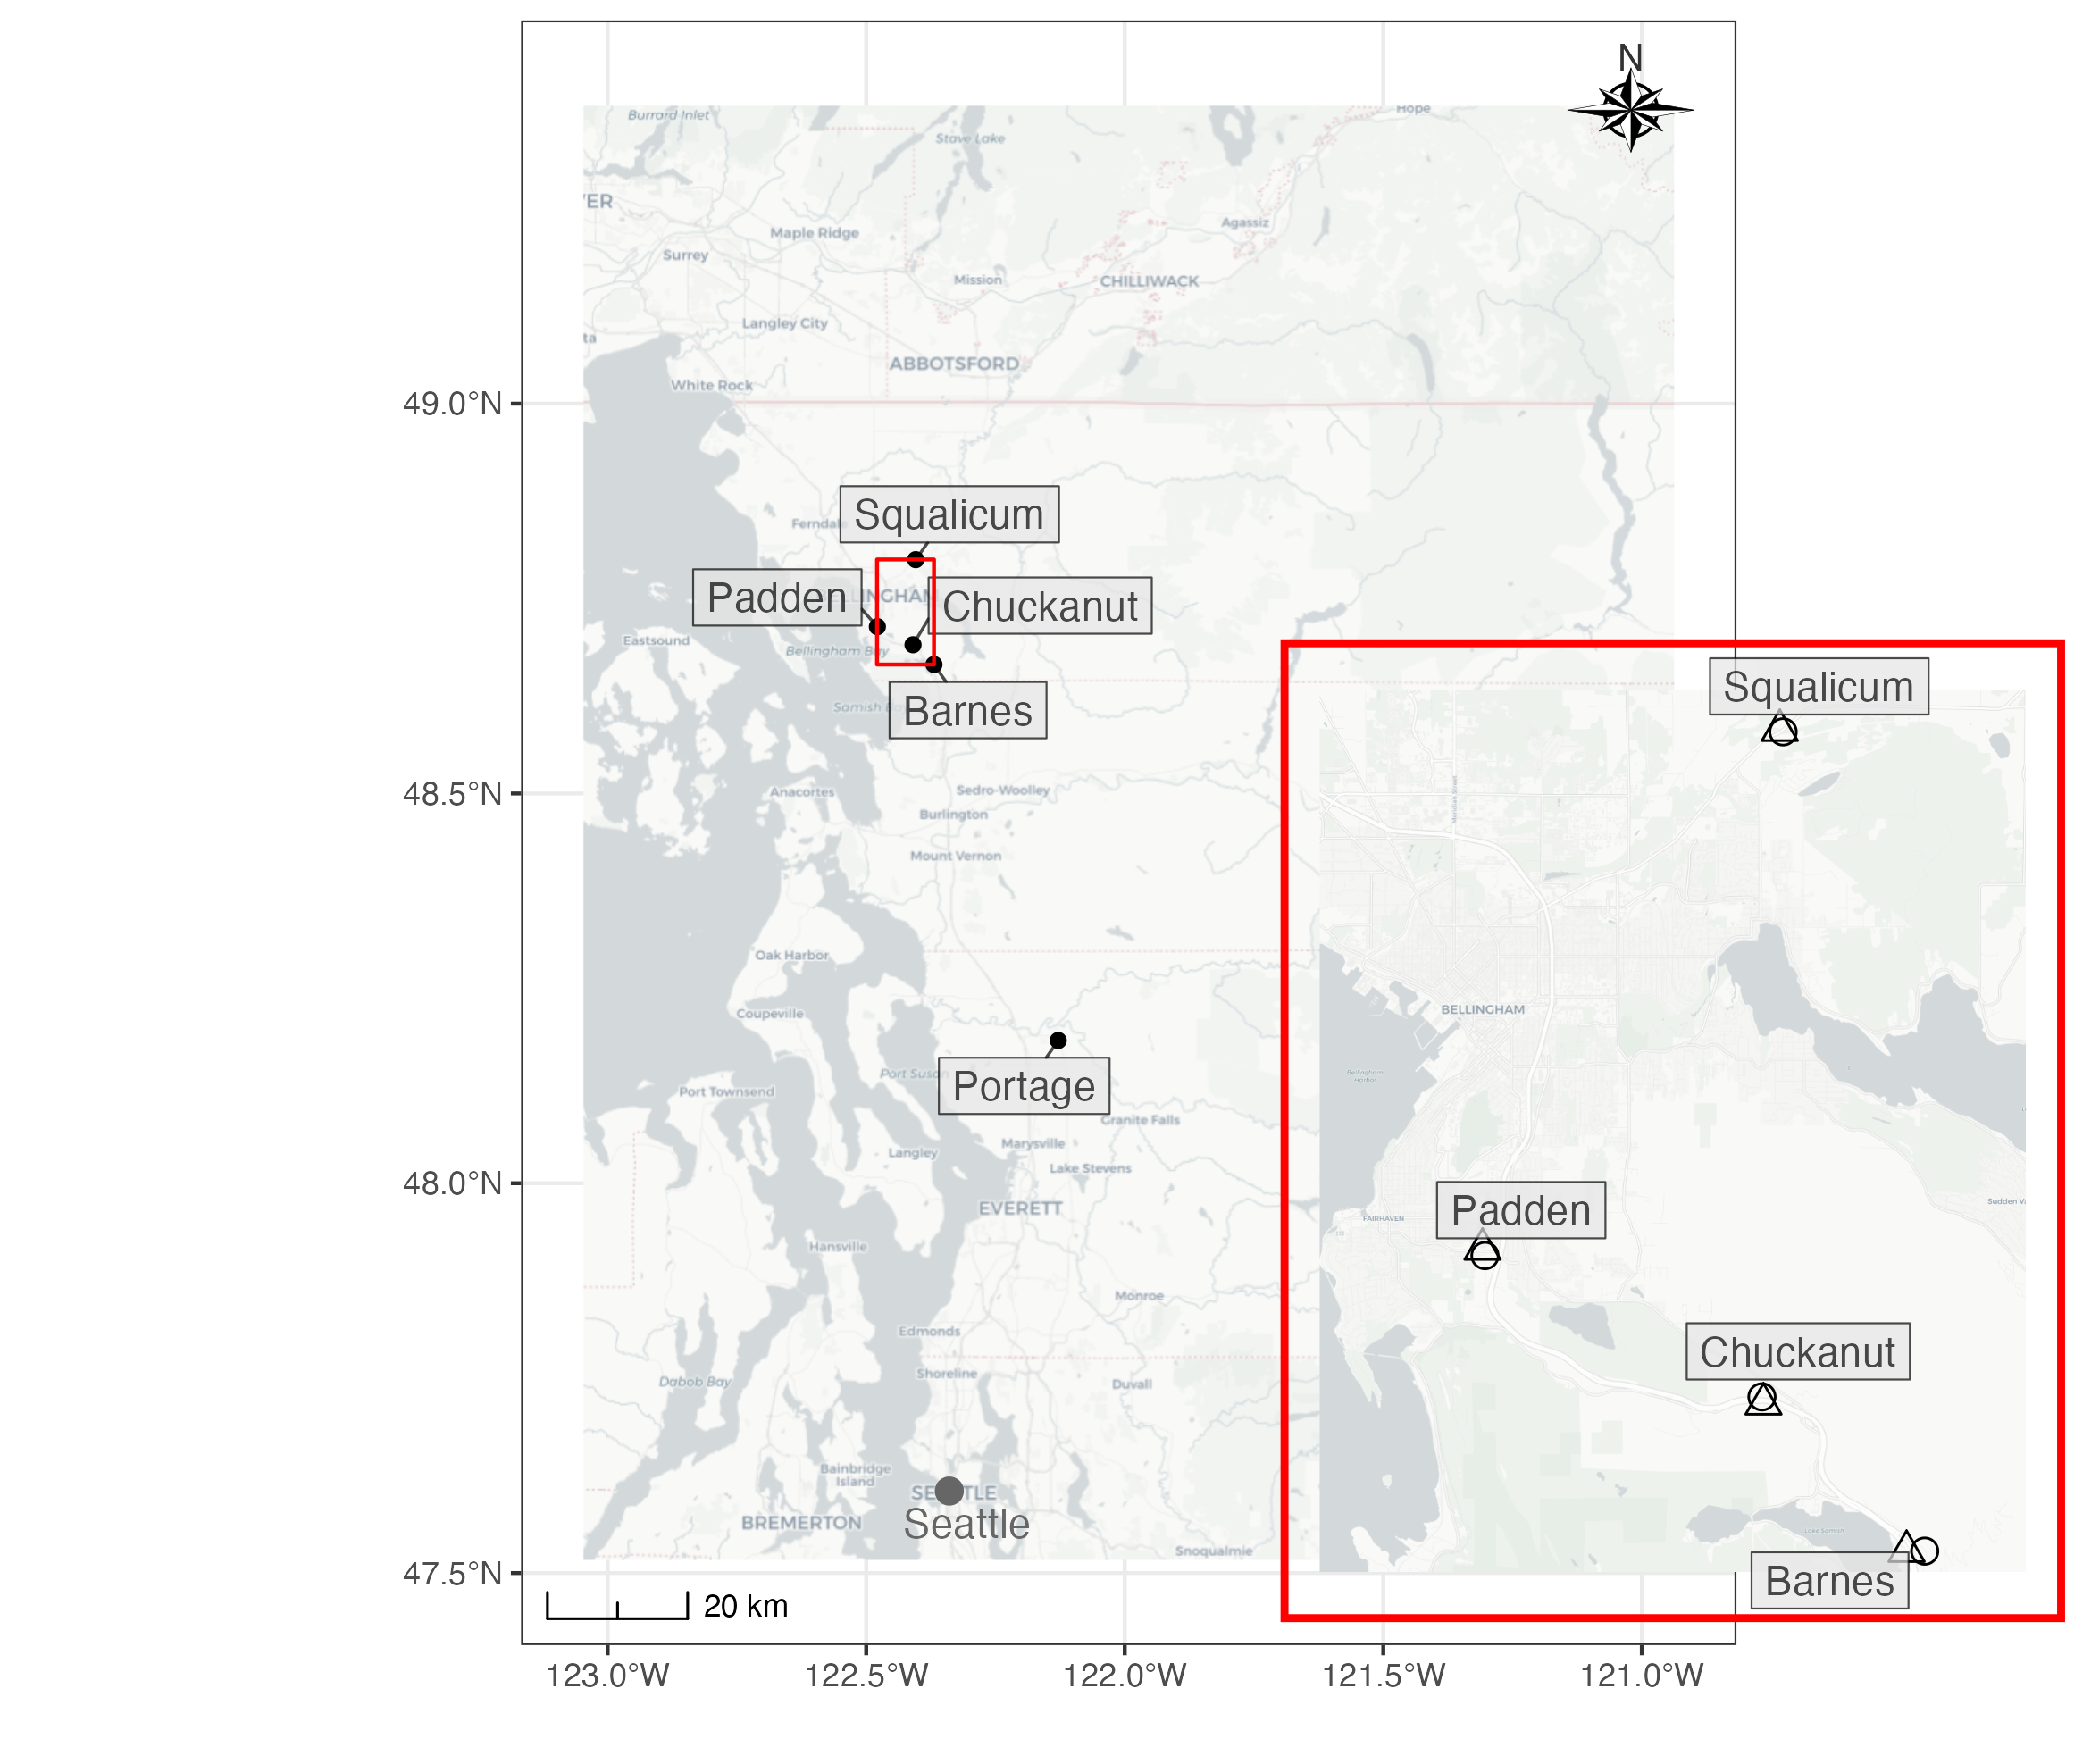
\includegraphics[width=0.5\textwidth,height=\textheight]{../Output/Figures/SiteMap.png}
\caption{Map of sampling locations near Bellingham, Washington.}
\end{figure}

Water samples were collected using Smith Root's eDNA Backpack
{[}CITE{]}, a portable pumping-and-filtering device set to filter at 1
L/min at 82.7 kPa (12 psi). In some months, less than 2 L of water was
filtered due to clogging (Supplemental Table X). Water samples were
filtered through 5\(\mu\)m self-preserving filters (Smith Root,
Vancouver, WA) using single-use inlet tubes, dried, and kept at room
temperature until DNA extraction within 1 month of collection (CITE
self-preserving filter paper).

Water discharge varied throughout the year, with lowest discharge in
summer months and highest discharge in winter months. Flow gauges
maintained by USGS were used for Padden Creek, Chuckanut Creek, and
Squalicum Creek. During the year of sampling, the flow gauges at
Chuckanut Creek and Squalicum Creek stopped metering after a major
flooding event. To find discharge rates for each creek to correct eDNA
concentrations by discharge, five years of historical data (2015-2020)
of the three creeks were used to generate a monthly averaged correction
factor based on Padden Creek. For the year of sampling (2021-2022), the
discharge rates used at Chuckanut and Squalicum Creeks were estimated
based on the correction factor from Padden Creek. No discharge data was
available for Portage Creek or Barnes Creek. Based on field sampling
conditions, the discharge from Padden Creek was used as a proxy for both
Portage and and Barnes as they were similar sizes and flow rates. Though
in the year of sampling, the discharge in Padden Creek ranged from no
metered flow to 23 m\textsuperscript{3}/s, the discharge on the dates of
sampling only reached a maximum of 1.3 m\textsuperscript{3}/s.

\begin{figure}
\centering
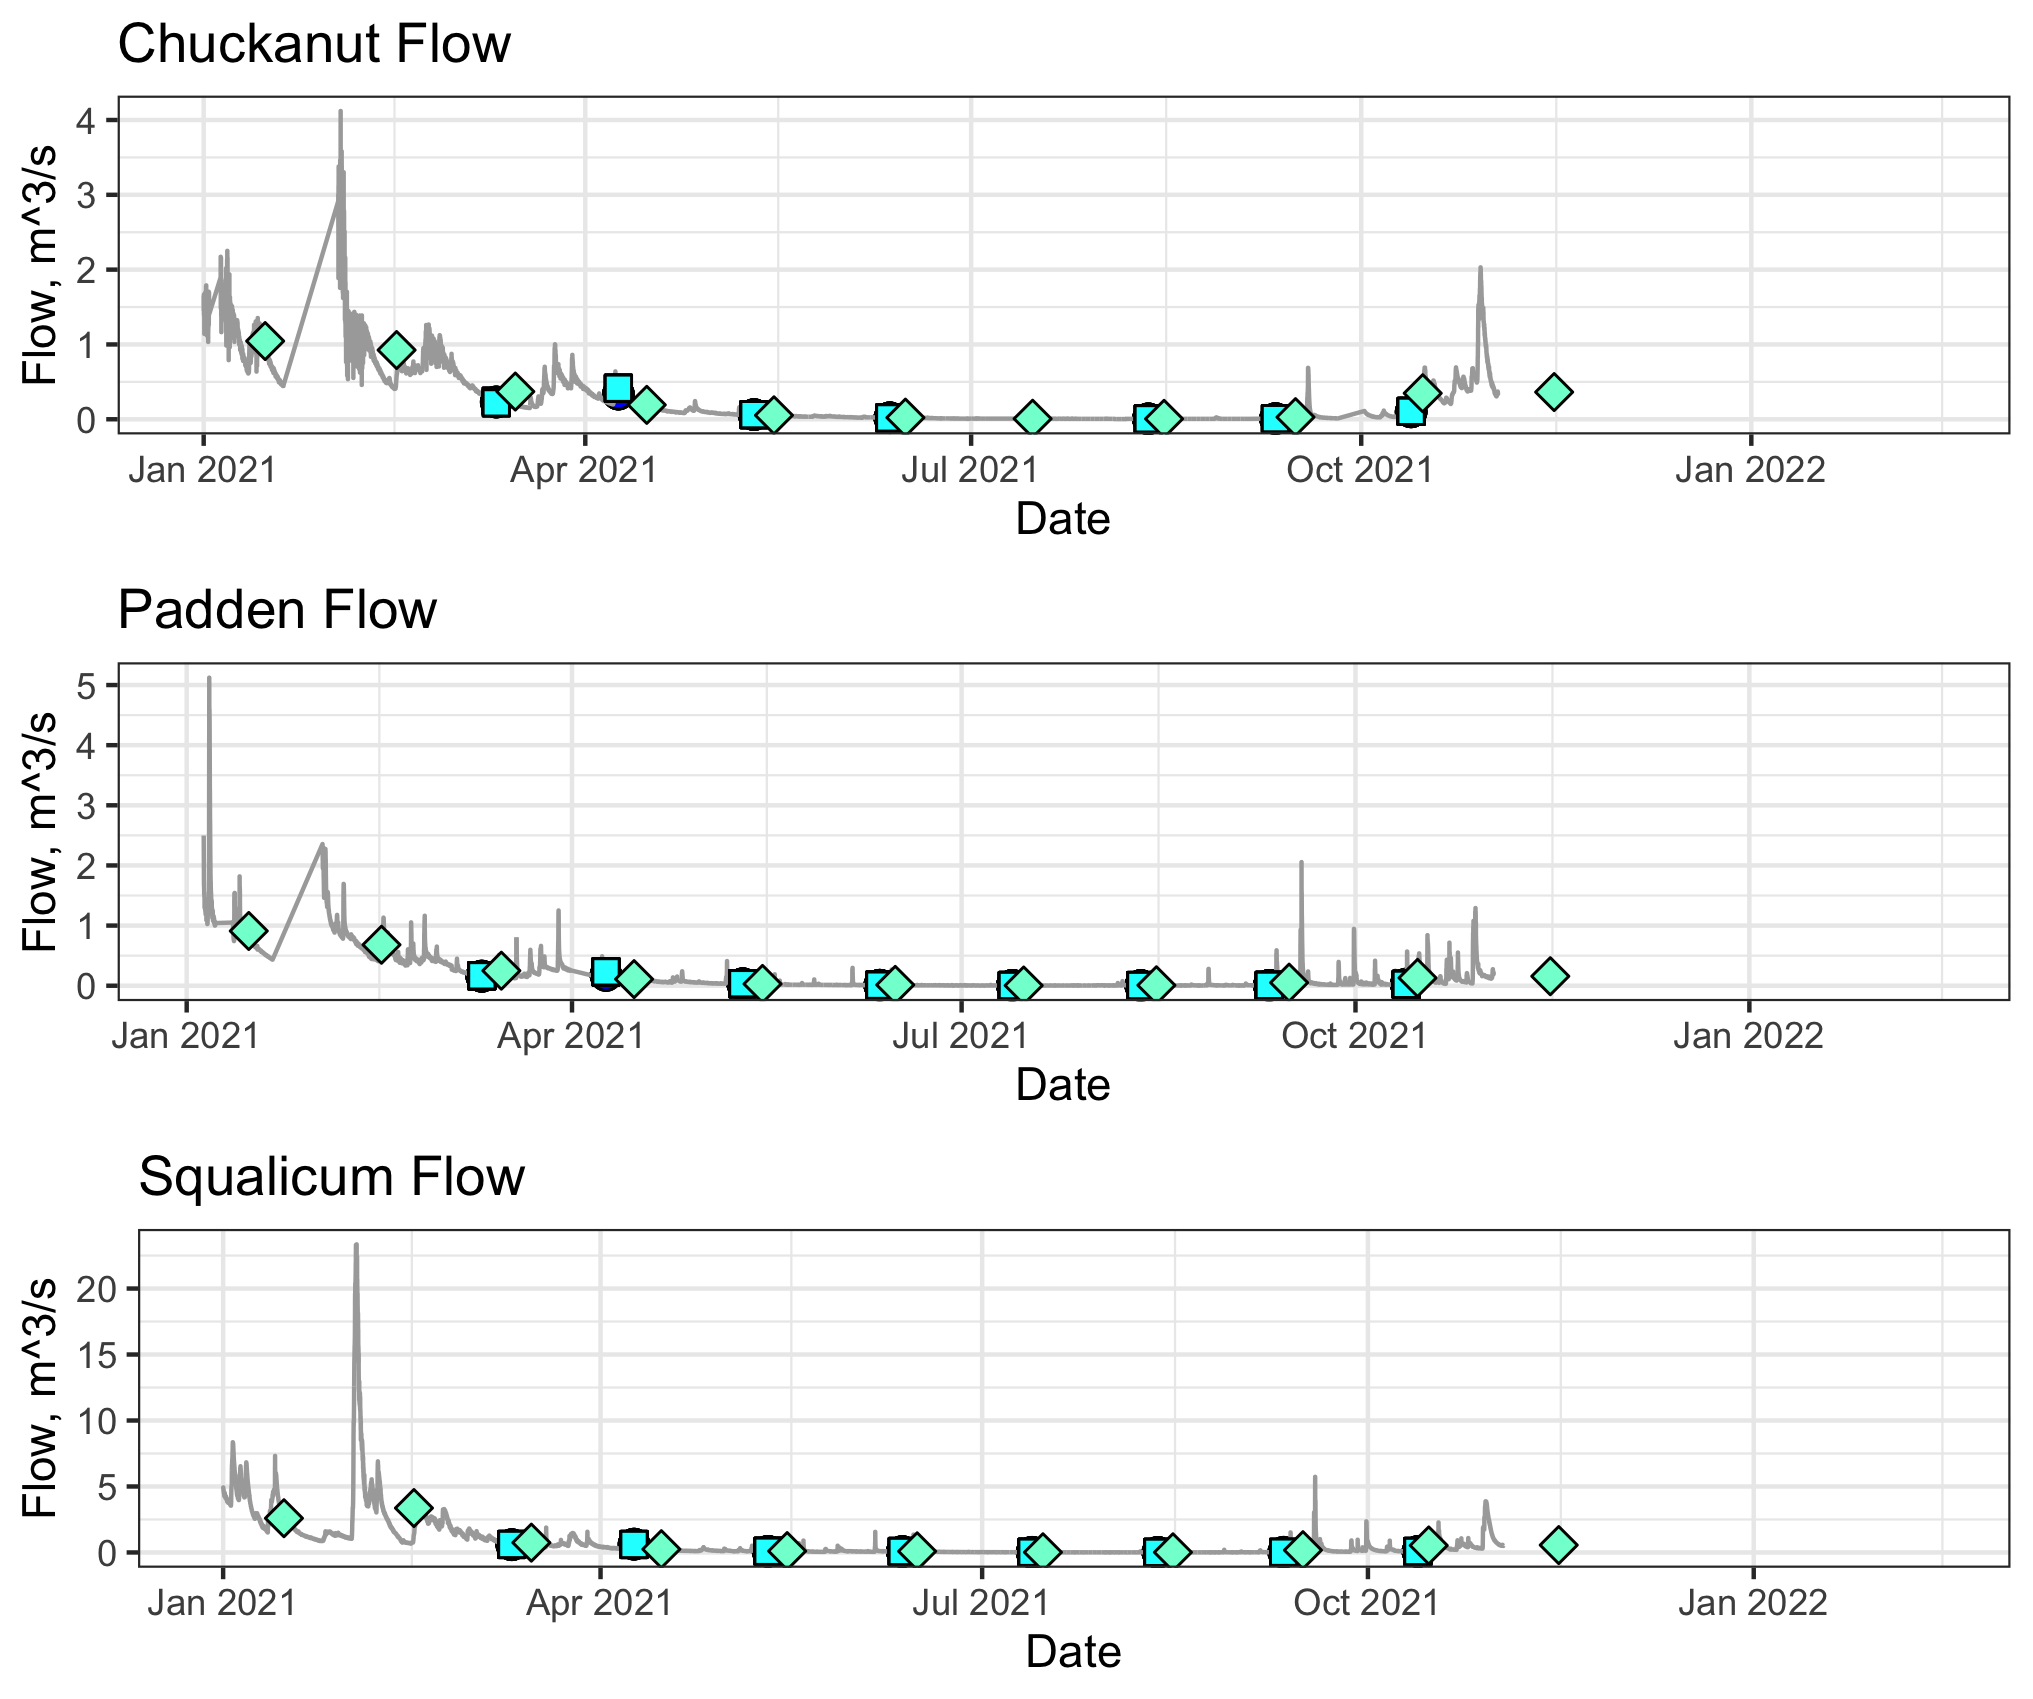
\includegraphics[width=0.7\textwidth,height=\textheight]{../Output/Figures/flow_gauges.png}
\caption{Discharge (m\textsuperscript{3}/s) in Padden, Chuckanut, and
Squalicum Creeks over the course of sampling. Open circles show the days
when sampling occurred. Gauges at Chuckanut and Squalicum Creek went
offline in November 2021 after a major storm event.}
\end{figure}

Additionally, in the creek of interest, Padden Creek, \emph{O. mykiss}
(rainbow trout) were stocked in Lake Padden, approximately 1.5 km
upstream of the sampling sites. Occasionally, cutthroat trout (\emph{O.
clarkii}) and kokanee salmon (\emph{O. nerka}) have been stocked in the
past as well. During the course of the study, a total of 10,000 rainbow
trout were stocked in April and May 2021, 30,000 kokanee salmon were
stocked in May 2021, and 10,000 cutthroat trout were stocked in January
2021 (Supplemental Figure X).

\hypertarget{dna-extraction-amplification-sequencing}{%
\subsubsection{DNA Extraction, Amplification,
Sequencing}\label{dna-extraction-amplification-sequencing}}

All molecular work was performed at the University of Washington.
Benchtops were cleaned with 10\% bleach for 10 minutes and then wiped
with 70\% ethanol. Molecular work was separated onto pre- and post-PCR
benches; all DNA extractions and PCR preparation was conducted on a
bench where no PCR product was handled.

We extracted DNA from half of each filter using a Qiashredder column
(Qiagen, XX) and the DNEasy Blood and Tissue Kit (Qiagen, XX) with an
overnight incubation (Supplement X), such that the effective filtering
effort was 1L/sample; the remaining half of each filter was archived at
-20\degree C. Extracts were eluted in 100 uL of molecular grade water,
quantified via Qubit (Invitrogen, XX) and stored at -20\degree C until
PCR amplification within X months of extraction (check longest time
waited).

We targeted a \textasciitilde170 bp hypervariable region of the
mitochondrial DNA 12S rRNA gene for PCR amplification (MiFish; CITE Miya
et al.), but using modified primer sequences as given in Praebel and
Wangensteen {[}cite{]} and including the Illumina Nextera overhang
sequences for subsequent indexing. The primers used were as follows: F
5' \emph{TCGTCGGCAGCGTCAGATGTGTATAAGAGACAG}GCCGGTAAAACTCGTGCCAGC 3', R
5' \emph{GTCTCGTGGGCTCGGAGATGTGTATAAGAGACAG}CATAGTGGGGTATCTAATCCCAGTTTG
3' (italics indicates Nextera overhang). The final reaction recipe and
cycling conditions are in Supplement X. Each month of samples was
amplified on a single plate with the addition of a no template control
(NTC; molecular grade water in lieu of template) and a positive control
(genomic DNA from kangaroo). After PCR amplification, PCR products were
visualized on a 1-2\% gel. If no band was present for a given sample, a
new amplification was attempted with extracts diluted 10x iteratively
until a band was detected. PCR products were size-selected and cleaned
using MagBind Beads (Omega Biotek, XX) at a sample:beads ratio of 1.2.
Bead-cleaned PCR products were eluted in 30 \(\mu\)L of molecular grade
water and quantified via Qubit (Invitrogen, XX).

A indexing PCR reaction added a unique index to each sample using
Nextera indices (Illumina, XX) to allow pooling multiple samples onto
the same sequencing run (See Supplement X for details). Indexed PCR
products were also size-selected and purified using MagBind Beads (Omega
Biotek, XX) at a sample:beads ratio of 0.8. Bead-cleaned PCR products
were eluted in 30 \(\mu\)L of molecular grade water and quantified via
Qubit. Indexed and bead-cleaned products were normalized before pooling
into libraries, which were subsequently quantified via Qubit and
visualized on a Bioanalyzer (Agilent, XX) before sequencing. Samples
were randomized in 3-month blocks and each block split across 3
sequencing runs, for a total of 12 MiSeq runs. The loading concentration
of each library was 4 nM and 5-20\% PhiX was included depending on the
composition of the run (Supplemental Table X).

In total, sequencing runs generated \textasciitilde42 million reads
across XX environmental samples (12 months x 2 stations x 5 creeks x 3
biological replicates = 360 filters) and 27 mock community samples (3
communities x 9 replicates {[}6 even, 3 skewed proportions{]}) for
calibration (see below). After quality-filtering and merging all runs,
XX reads remained from XX amplicon sequence variants (ASVs), of which
XX\% of reads and XX\% of reads were annotated to species level.

Importantly, the particular target salmonid ASVs in the mock communities
were found in environmental samples, unambiguously linking the taxa in
calibration samples with those in environmental samples. The most common
salmonid species found in the environmental samples was \emph{O.
clarkii} (cutthroat trout), with XX\% of samples across times, creeks,
and stations having at least 50\% of reads assigned to \emph{O.
clarkii}.

\hypertarget{bioinformatics}{%
\subsubsection{Bioinformatics}\label{bioinformatics}}

After sequencing, bioinformatic analyses were conducted in R {[}cite
R{]}. Information about the bioinformatics pipeline is included in the
Supplemental Methods. Briefly, primer sequences were removed using
Cutadapt (Version 1.18) {[}cite cutadapt{]} before dada2 {[}cite{]}
trimmed, filtered, merged paired end reads, and generated amplicon
sequence variants (ASVs). Taxonomic assignment was conducted via the
insect package {[}cite{]} using a tree generated by the developers for
the MiFish primers that was last updated in November 2018. Only species
level assignments from insect were retained and ASVs not annotated or
not annotated to species level were then checked against the NCBI
nucleotide database using BLAST+ {[}cite{]}. Query sequences that
matched a single species at \textgreater95\% identity were retained.

From all the ASVs generated from environmental samples, a total of X
unique ASVs were found, with X\% of ASVs (representing X\% of reads)
assigned to species level (Supplemental Table X). Only reads assigned to
the four salmonids of interest were retained for further analysis, which
was X\% of reads.

\hypertarget{quantitative-pcr-and-inhibition-testing}{%
\subsubsection{Quantitative PCR and Inhibition
Testing}\label{quantitative-pcr-and-inhibition-testing}}

We quantified cutthroat trout (\emph{O. clarkii}) DNA in each sample,
targeting a 114 bp fragment of the cytochrome b gene with a qPCR assay
(CITE-- Duda?). The primer/probe sequences were: F 5'
CCGCTACAGTCCTTCACCTTCTA 3', R 5' GATCTTTGTATGAGAAGTAAGGATGGAA 3', P 5'
6FAM-TGAGACAGGATCCAAC-MGB-NFQ 3'. The qPCR assay was multiplexed with
TaqMan Exogenous Internal Positive Control Reagents (EXO-IPC) (Applied
Biosystems) to check for the presence of PCR inhibitors. Each DNA sample
was run in triplicate; the final recipe and thermocycling conditions can
be found in Supplelment X. The EXO-IPC mix includes the primers and
probe for the EXI-IPC DNA, with the probe having a VIC reporter,
allowing it to be multiplexed with the \emph{O. clarkii} assay, which
has a FAM reporter. All qPCRs were conducted on an Applied Biosystems
StepOnePlus thermocycler.

Each plate included a 8-point standard curve created using synthetic DNA
(gBlocks) at the following concentrations: 100,000 copies/\(\mu\)L,
10,000 copies/\(\mu\)L, 1,000 copies/\(\mu\)L, 100 copies/\(\mu\)L, 10
copies/\(\mu\)L, 5 copies/\(\mu\)L, 3 copies/\(\mu\)L, 1 copy/\(\mu\)L
Additionally, six NTCs were included on each plate: 3 with the IPC DNA
mix and 3 with molecular grade water instead of template or IPC DNA mix.
Plates were re-run if efficiency as determined by the standard curve was
outside of the range of 90-110\%.

To check for inhibition, the cycle threshold (Ct) value determined for
the EXO-IPC assay from the NTC was compared to the Ct value for the
EXO-IPC assay in each of the environmental samples. If the Ct value was
\textgreater0.5 Ct values from the mean Ct for the NTCs, the sample was
deemed inhibited and diluted 1:10 and re-assayed until the Ct value fell
within the accepted range. The majority of environmental samples (65\%)
were inhibited and accordingly diluted for analysis. In 75\% of
inhibited samples, a 1:10 dilution remedied the inhibition, but some
samples required dilution by a factor of up to 1000.

All qPCR data was processed in R using Stan, relating environmental
samples to the standard curve via a linear model (Figure 2, blue boxes).
We amended the standard linear regression model to more realistically
capture the behavior of qPCR observations, accommodating non-detections
as a function of underlying DNA concentration, and letting the standard
deviation vary with the mean (lower-concentration samples had more
uncertainty).See also See Shelton et al.~2019; McCall et al.~2014
(\url{https://www.ncbi.nlm.nih.gov/pmc/articles/PMC4133581/}); see
supplement for full statistical details. Subsequent analysis corrected
for sample-specific dilution if found inhibited -- and similarly, any
variation in water-volume filtered during sample collection.

\hypertarget{quantitative-metabarcoding}{%
\subsubsection{Quantitative
Metabarcoding}\label{quantitative-metabarcoding}}

Here, we used a mock community to determine the species-specific
amplification efficiencies for each salmonid in the study. Briefly, we
constructed three communities with known proportions of starting DNA
from different species (total DNA as measured by Qubit). Each community
was constructed with an even proportion of each species and a skewed
proportion. We sequenced these communities using the same metabarcoding
primers and thermocycling conditions above and then can determine the
species-specific amplification rates given the discrepancy between the
known starting proportion and the proportion of reads after sequencing.
These mock community data are then used to correct the sequencing reads
from the environmental samples to estimate the starting DNA proportions
of each species in environmental samples, which is the metric of
interest (Figure 2, green boxes). See Shelton et al.~2022 and the
Supplemental Materials for more information. The intercalibration of the
mock community samples demonstrates the rank order of ampliciation
efficiencies for salmonids (Supplemental Figures X and Y). \emph{O.
clarkii} and \emph{O. nerka} had similar amplification efficiencies,
both of which were higher than \emph{O. mykiss} and \emph{O. kisutch},
which had the lowest amplification efficiency.

Calibrated metabarcoding analysis yielded quantitative estimates of the
proportions of species' DNA in environmental samples prior to PCR. We
then converted these proportions into absolute abundances by expansion,
in light of the qPCR results for our reference species \emph{O.
clarkii}. We estimated the total amplifiable salmonid DNA in
environmental sample \(i\) as
\(DNA_{salmonid_{i}} = \frac{[qPCR_{reference_{i}}]}{Proportion_{reference_{i}}}\),
and then expanded species' proportions into absolute concentrations by
multiplying these sample-specific total concentrations by individual
species' proportions, such that for species \(j\) in sample \(i\),
\(DNA_{i,j} = DNA_{salmonid_{i}} * Proportion_{i,j}\). Finally, we
convert from DNA concentration {[}copies/L{]} to a mass flow rate
{[}copies/s{]} after multiplying by the discharge of each creek
{[}m\textsuperscript{3}/s{]} (Figure 2, solid purple boxes).

\begin{figure}
\centering
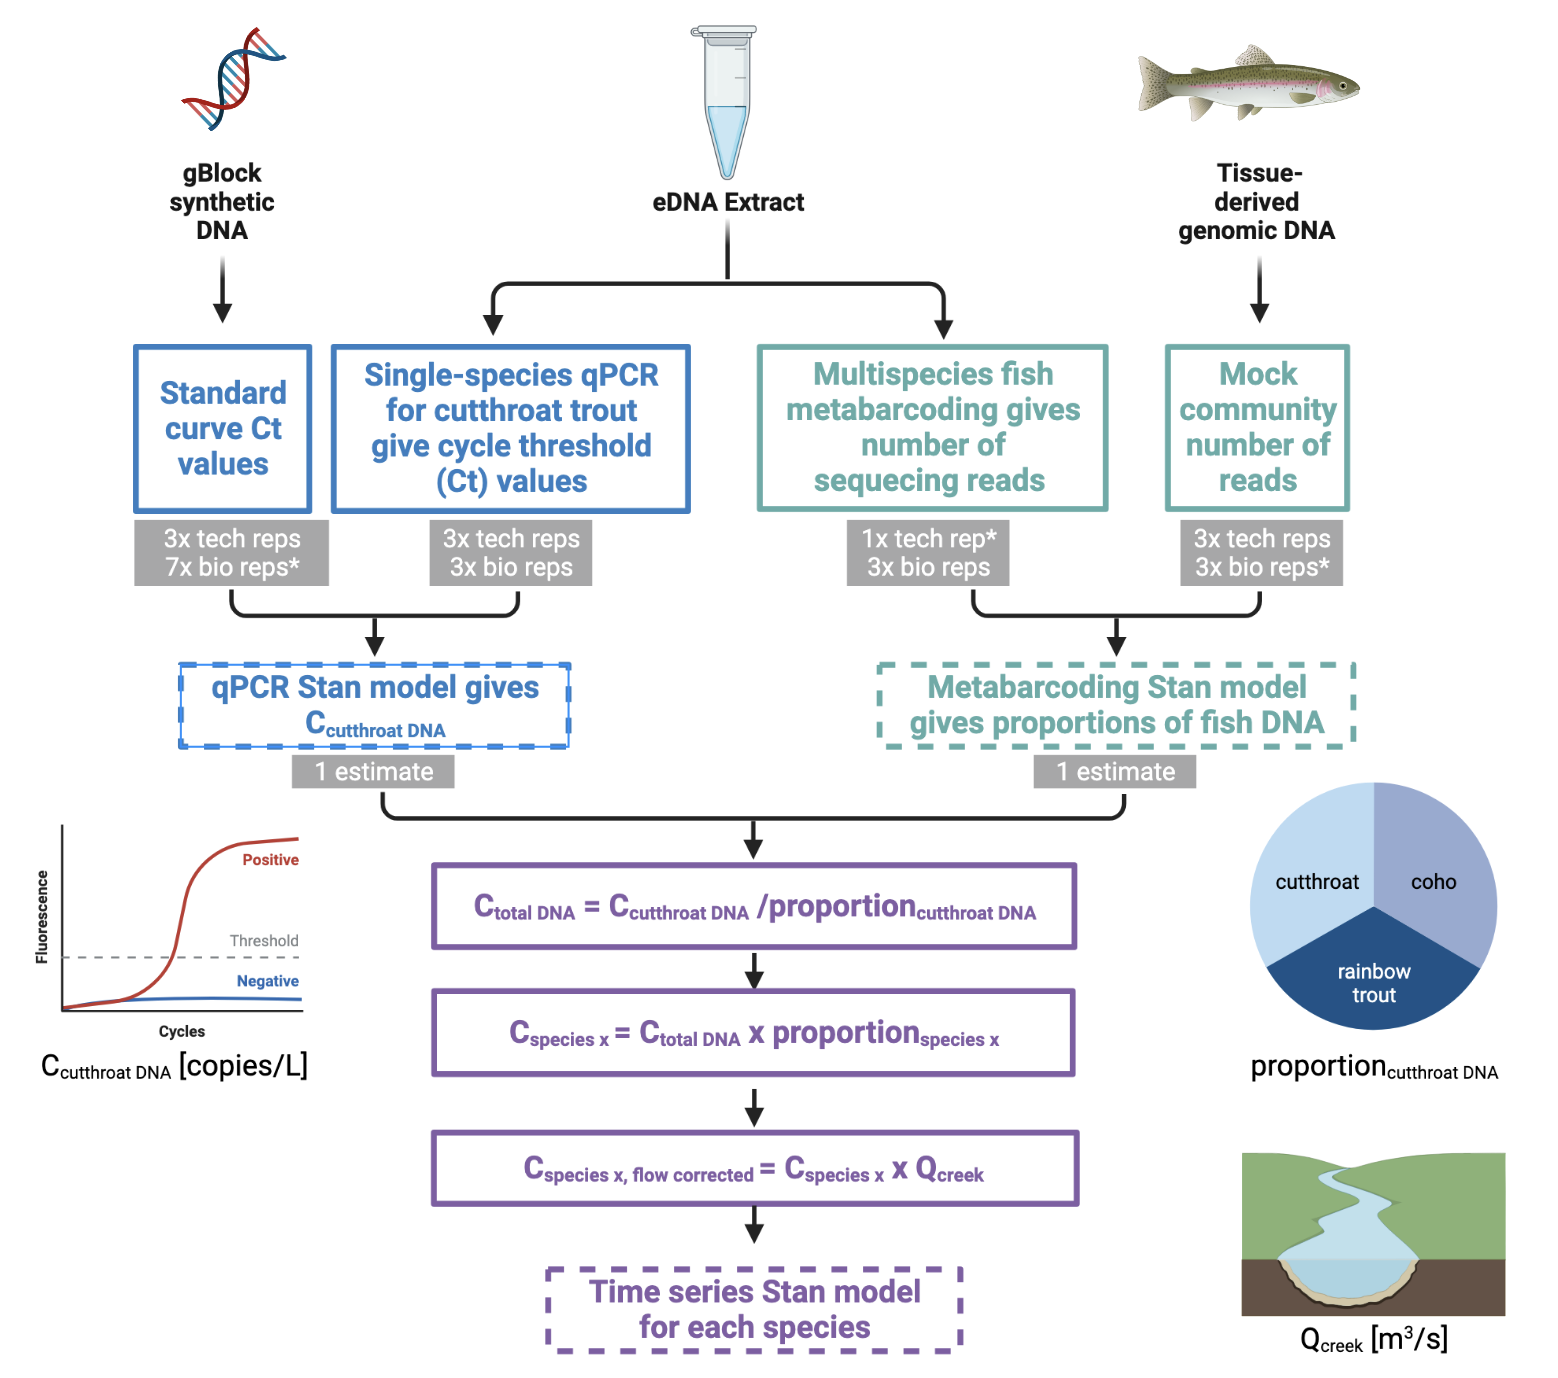
\includegraphics[width=0.75\textwidth,height=\textheight]{../Output/Figures/conceptual_figure.png}
\caption{Conceptual figure of different datasets and models used for
analyses.}
\end{figure}

\hypertarget{estimating-the-effects-of-culvert-replacement-and-of-culverts-themselves}{%
\subsubsection{Estimating the Effects of Culvert Replacement and of
Culverts
Themselves}\label{estimating-the-effects-of-culvert-replacement-and-of-culverts-themselves}}

Consistent with the asymmetrical BACI study design, we generated data
from our four control creeks as context against which to compare the
observations in Padden Creek, our treatment creek.

Recognizing that these observations are autocorrelated in time, we use
an AR(1) autocorrelation model, implemented in Stan via R, to capture
the observed temporal trends. At time \(t\), the expected log-DNA
concentration for species \(j\) in creek \(i\) at station \(d\) is a
linear function of the DNA concentration for the same
species/creek/station at \(t-1\) (Equation X). We add an index \(r\) to
distinguish samples from creeks and time-points that had not undergone
culvert replacement (controls; \(r = 1\)) from those samples in the
treatment creek during and post-replacement (treatment; \(r = 2\)).

\begin{align*}
 Y_{i,t,d,j} &\sim \mathcal{N}(\mu_{i,t,d,j},\,\sigma^{2})\\
\mu_{i,t,d,j} &= \alpha_{i,t,j} + \beta_{j}\mu_{i,t-1,d,j} + \gamma_{t,j,r} + \eta_{i,t,d,j}
\end{align*}

The model shares information across creeks and time-points via a
species-specific slope term \(\beta_{j}\), which reflects characteristic
degrees of autocorrelation for each species. Intercept \(\alpha\) varies
by time, creek, and species, capturing creek-level deviations from the
previous time-step.

The \(\gamma\) term explicitly captures the effect of culvert
replacement at time \(t\) for species \(j\). We define
\(\gamma_{r = 1} = 0\), such that the parameter estimates for samples
during and after replacement, \(\gamma_{r = 2}\), capture the effect of
culvert replacement relative to a baseline of zero.

Finally, for a given time/creek/species, the difference in log-DNA
concentration between upstream and downstream stations is calculated as
the difference between the parameter values of \(\eta\) for the two
stations. All samples share a species-specific observation-variance
term, \(\sigma_{j}\).

We fitted this model in a Bayesian framework using moderately
informative priors on all parameters, and confirmed model convergence
(\(\hat{R} < 1.01\)) across 3 chains and 2500 model iterations. See
statistical supplement for prior values, diagnostics, and full model
details.

\hypertarget{results}{%
\subsection{Results}\label{results}}

\hypertarget{metabarcoding-and-quantitative-pcr}{%
\subsubsection{Metabarcoding and Quantitative
PCR}\label{metabarcoding-and-quantitative-pcr}}

After calibrating metabarcoding data using mock communities, we
estimated the salmonid composition across time points, creeks, and
stations (Figure 3). The culvert in one control creek (Barnes) appeared
to be a total barrier to salmonid passage, with salmonid eDNA detected
upstream of the culvert at only three time points, in contrast to being
detected at every time point in the downstream station of the same
creek. The other four creeks had no such pattern associated with the
culverts, suggesting that fish passage may have been possible in each
case.

\begin{figure}
\centering
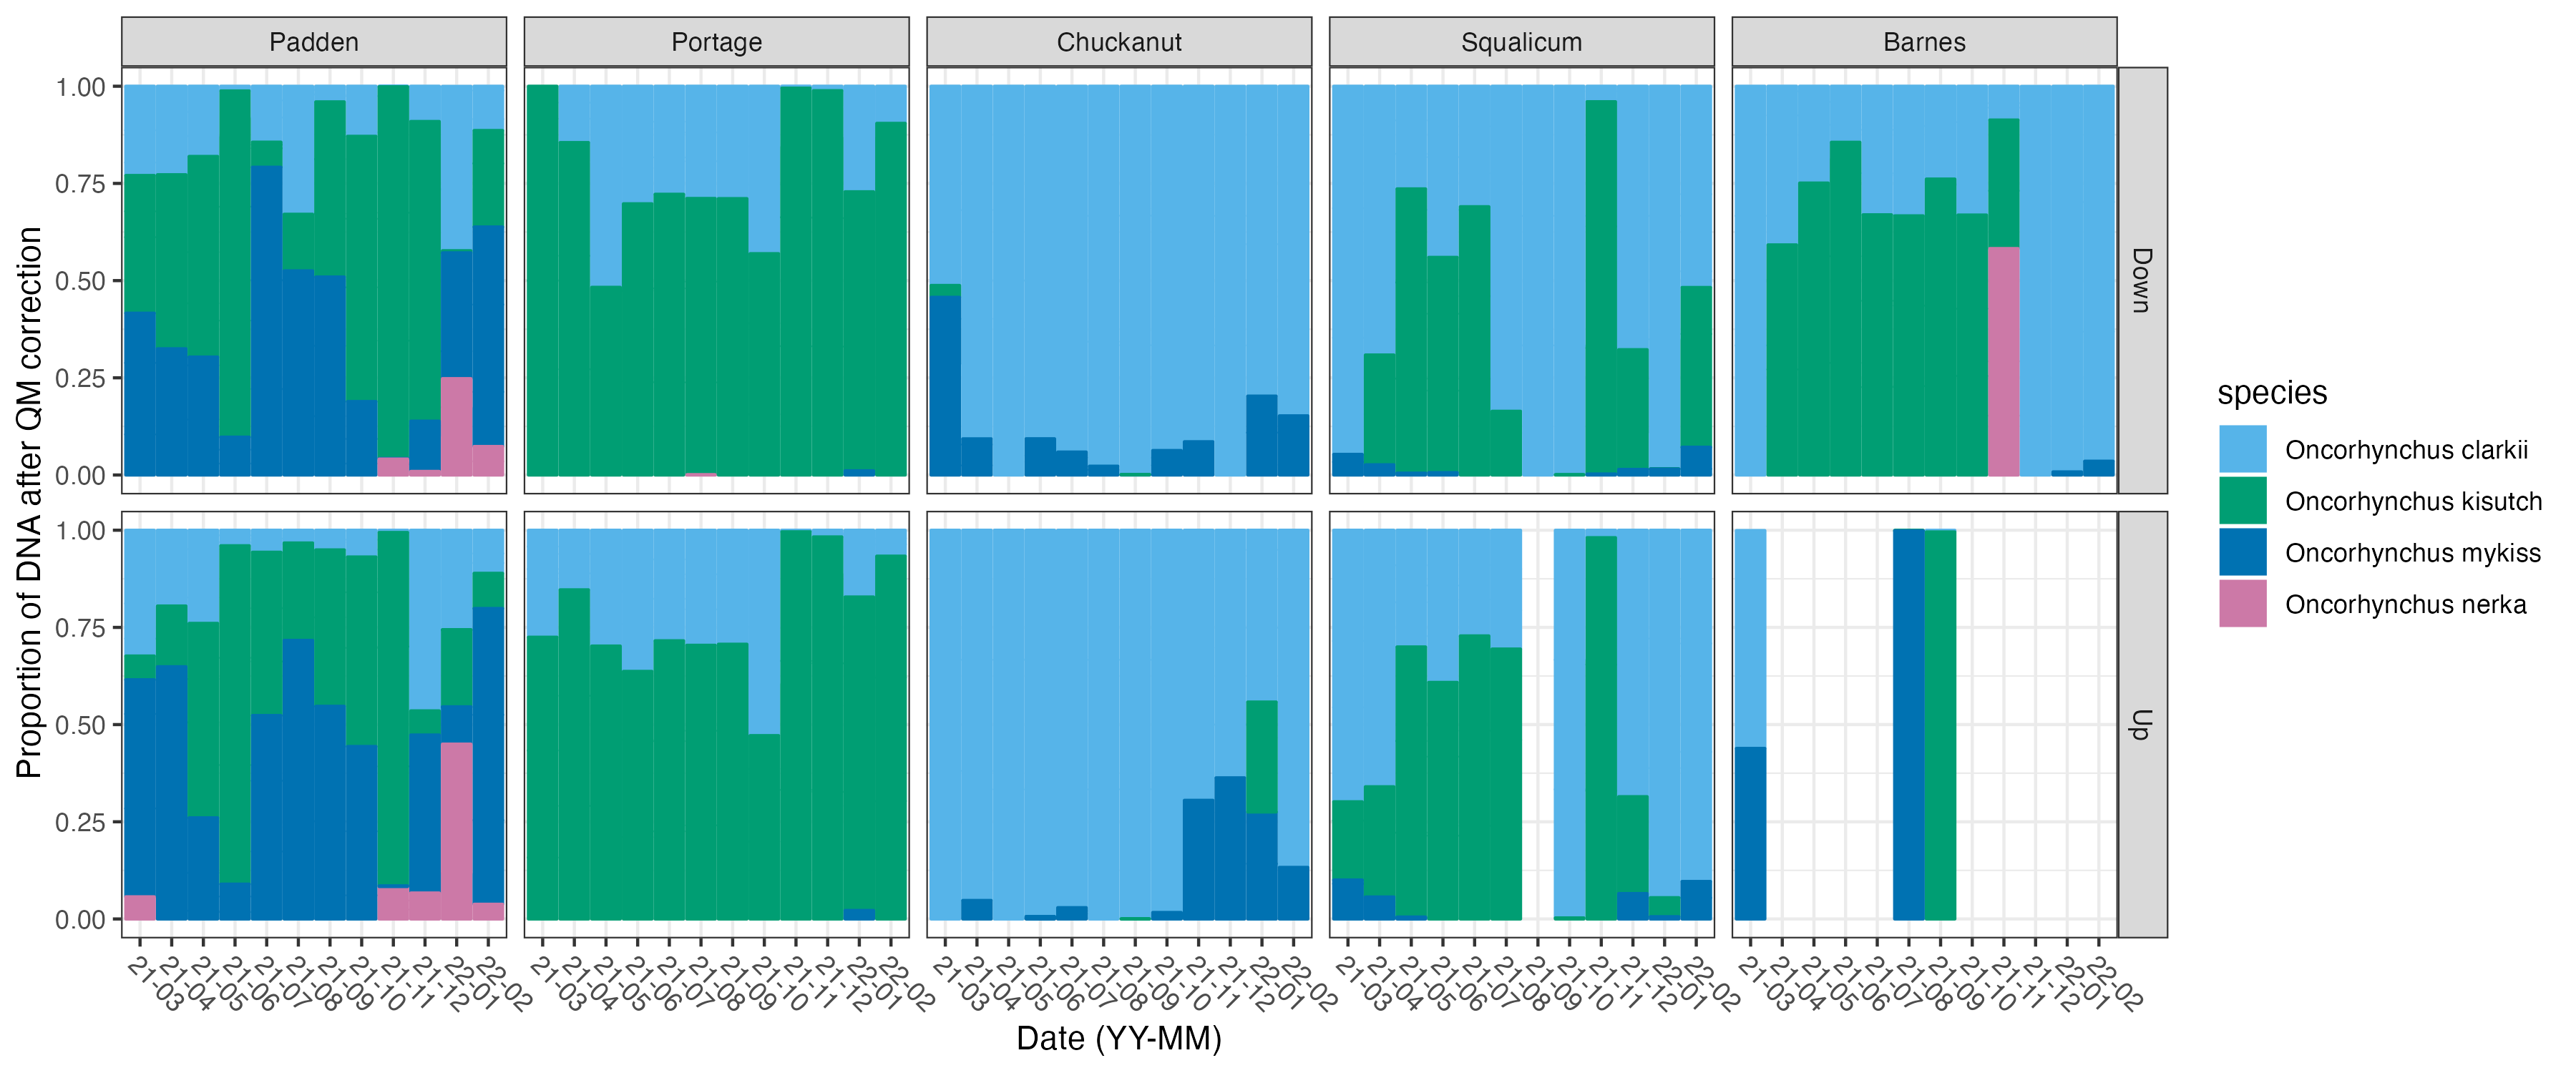
\includegraphics[width=0.9\textwidth,height=\textheight]{../Output/Figures/20221123_proportions_after_qm.png}
\caption{Compositions of salmonid DNA as determined by metabarcoding
after correction for amplification bias. Note that no sampling occurred
in September 2021 at Squalicum Creek becuase the creek was dry. The
empty bars in the Barnes upstream sites indicate that no salmonid DNA
was found at those time points.}
\end{figure}

All environmental samples (n = 356, should be 357, one set of
triplicates missing from Sqm Up August, otherwise 3x2x5x12 = 360) were
quantified for absolute concentrations of cutthroat trout DNA across 30
plates, resulting in 280 samples with a positive detection in at least 1
of 3 technical replicates. The modeled output of cutthroat trout DNA
concentrations, ranged from 10 copies/L to 1,377,656.67 copies/L, with a
mean value of 57,529 copies/L (Figure 4).

\begin{figure}
\centering
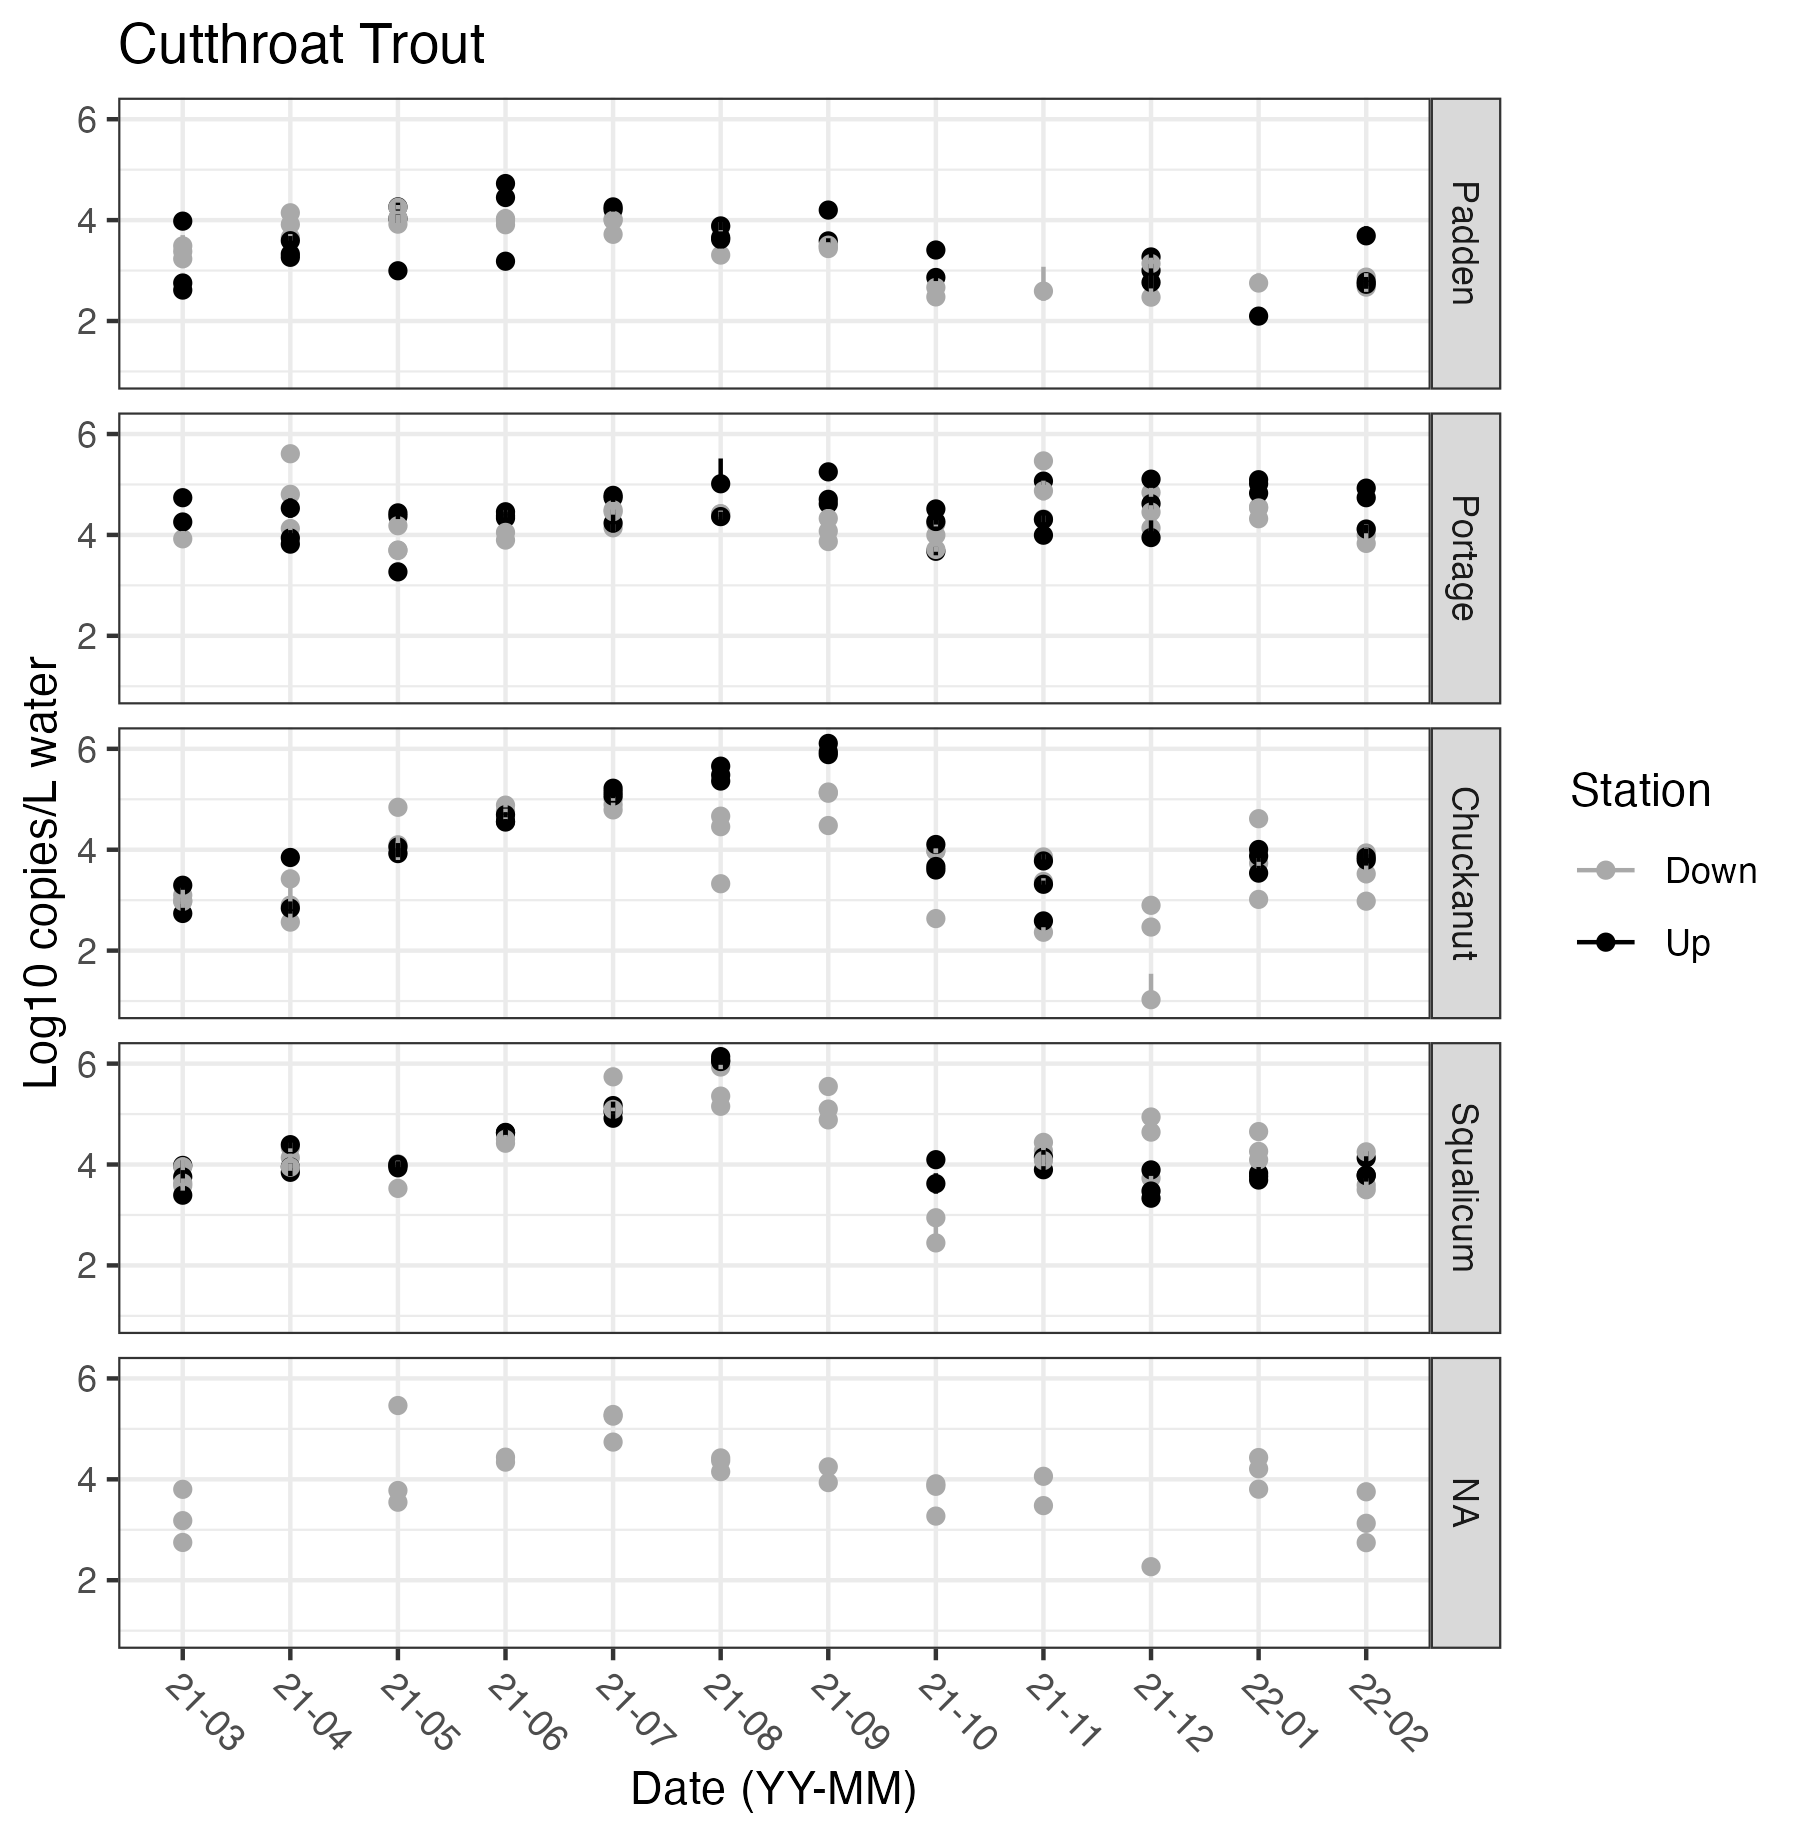
\includegraphics[width=0.6\textwidth,height=\textheight]{../Output/Figures/20221123_modeled_cut_qpcr_updown.png}
\caption{Absolute concentration (copies/L of water) of \emph{O. clarkii}
(cutthroat trout) as measured by qPCR.}
\end{figure}

We combined compositional information from metabarcoding with absolute
concentrations for our reference species, \emph{O. clarkii}, from the
qPCR to estimate the total concentration of DNA for each species. The
total DNA concentration of salmonid DNA in environmental samples ranged
from XX to XX copies/L (Supplemental Figure X), with the highest
concentrations found in X month and in X creek (Supplemental Figure X).

\hypertarget{trends-in-abundance}{%
\subsubsection{Trends in Abundance}\label{trends-in-abundance}}

The joint time-series model shared information across stations and
creeks; consequently, data from one of the control creeks (Barnes) could
not be included because of the total absence of salmonids upstream of
its culvert. However, data from the remaining creeks characterized
trends in the target species well (Figure 5).

\begin{figure}
\centering
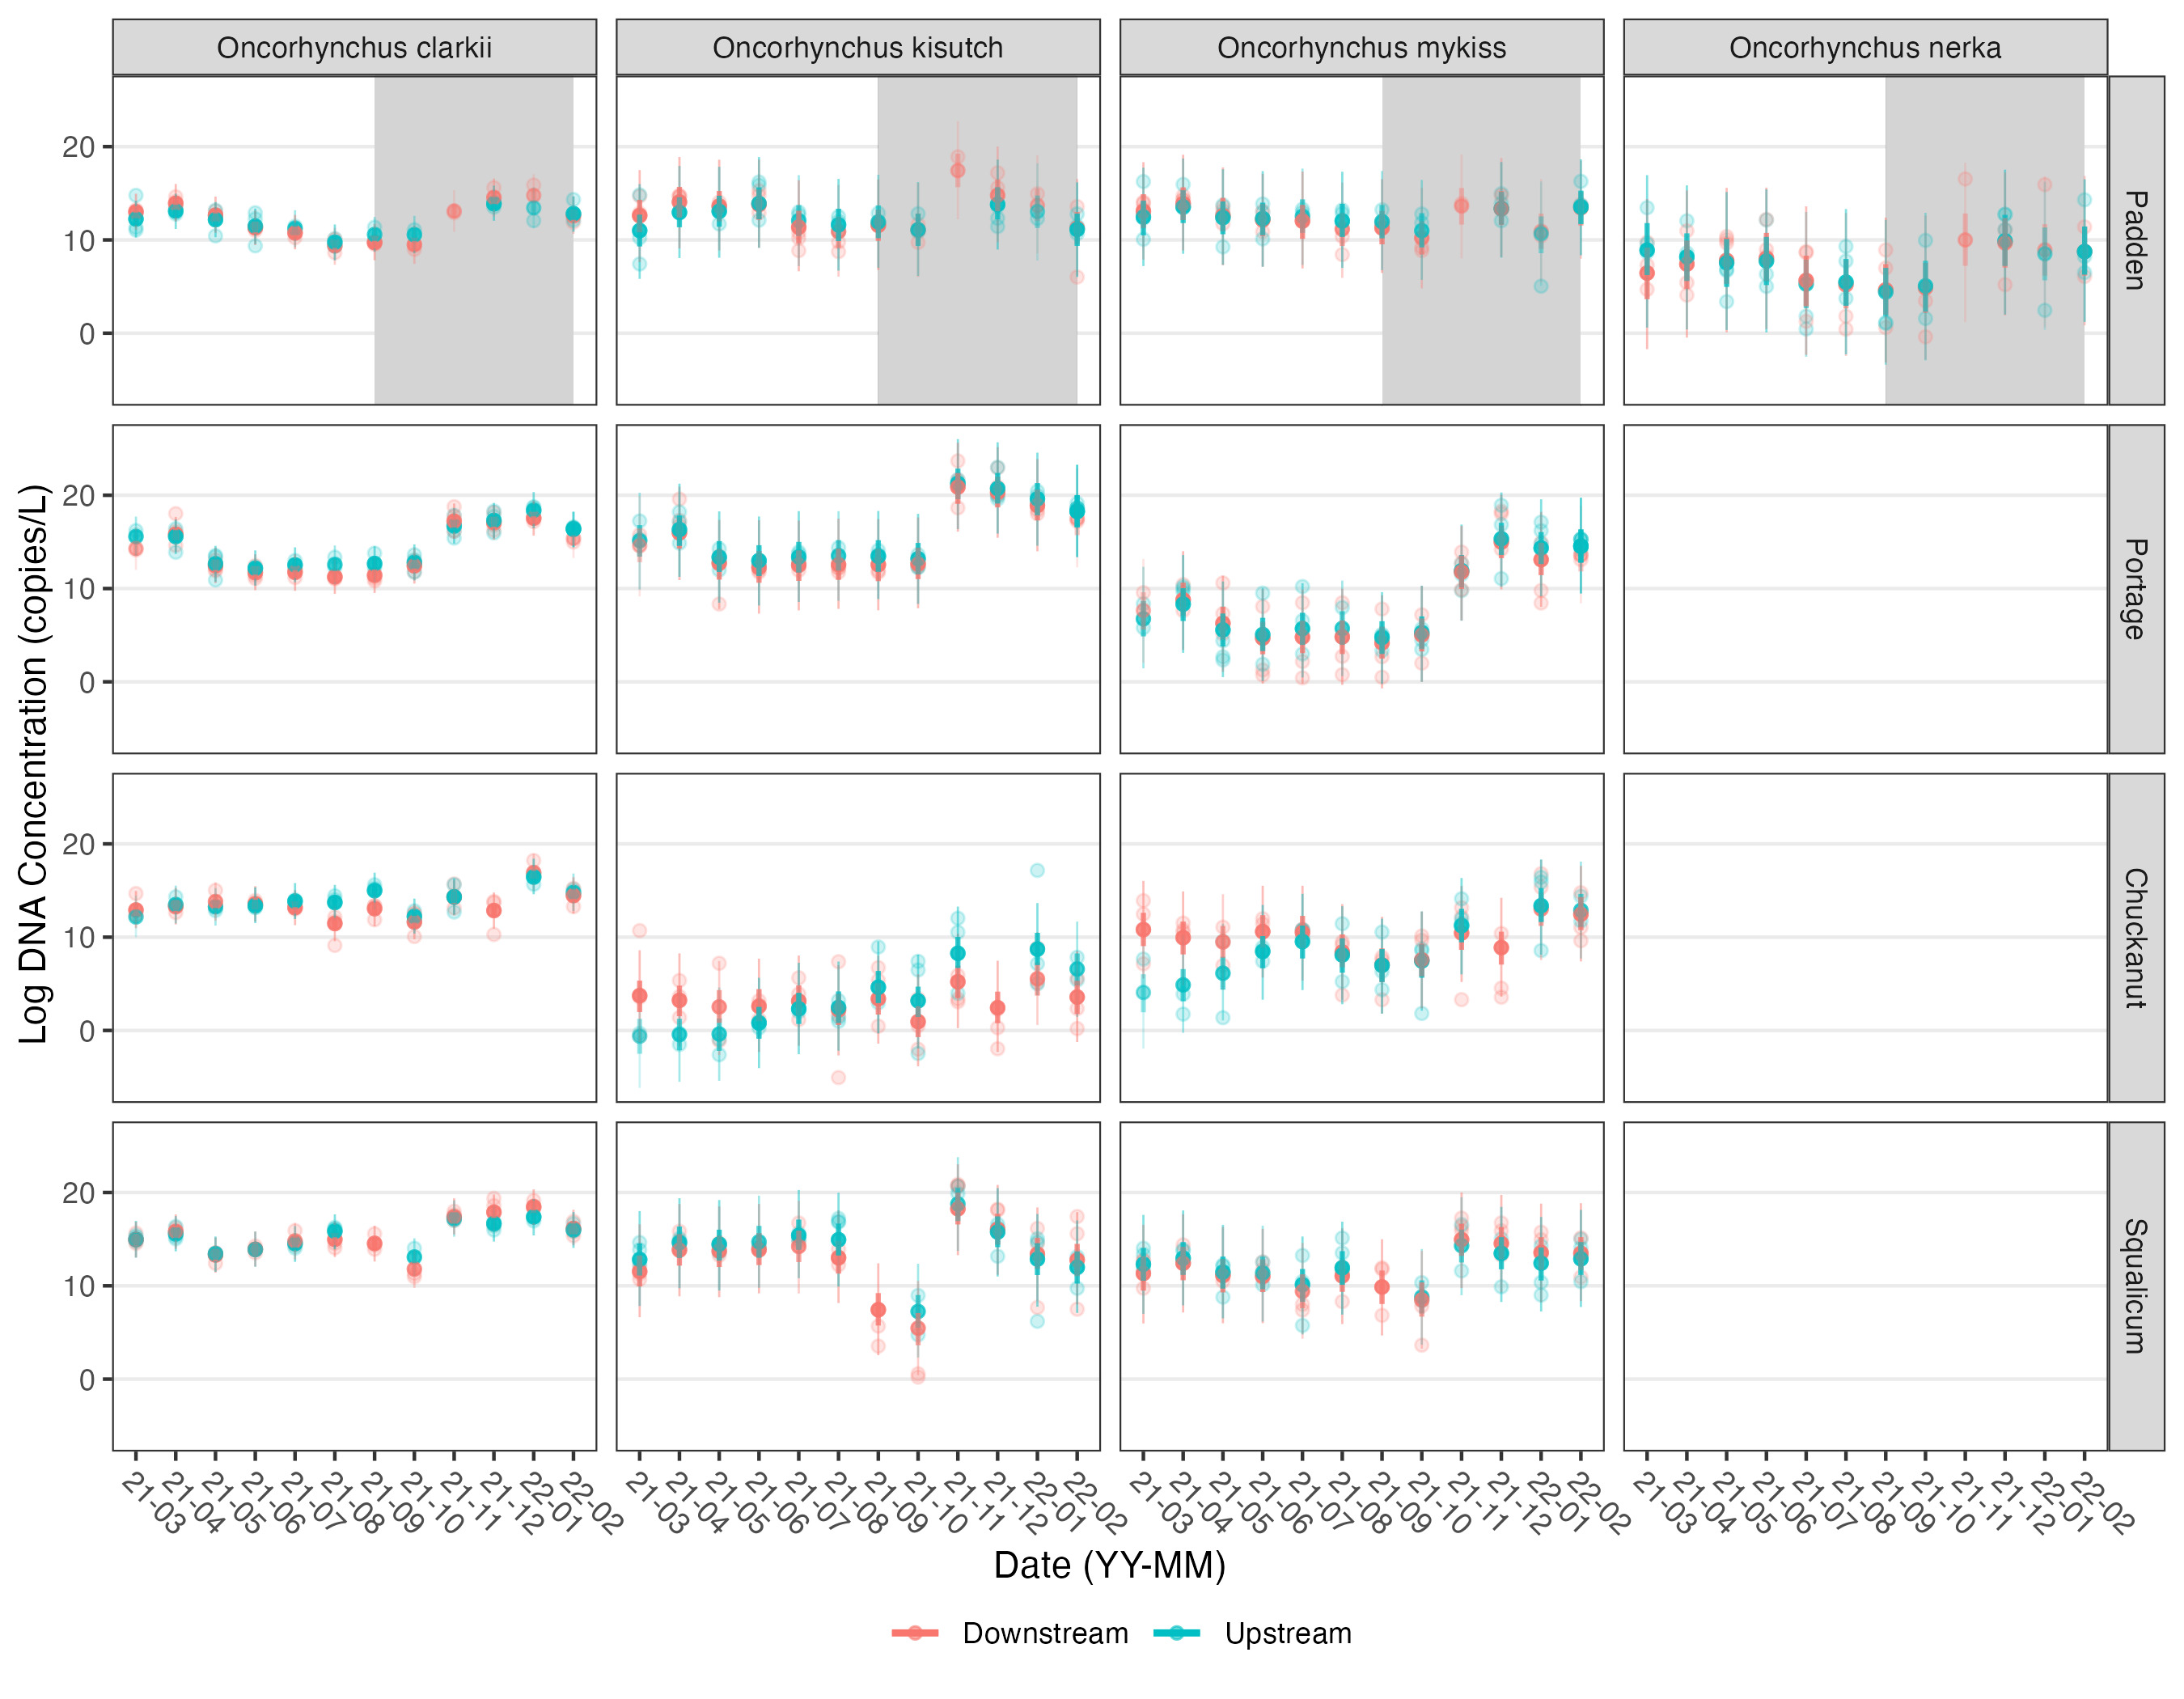
\includegraphics[width=0.75\textwidth,height=\textheight]{../Output/Figures/20221123_multispeciesTrends_flowcorrected.png}
\caption{Trends across creeks and across time for each of three salmonid
species as estimated by eDNA analysis. Light-colored dots are posterior
means derived by expanding the calibrated metabarcoding proportions as
described in the main text; darker-colored dots are posterior means for
the time-series model of the same. Colors indicate station upstream or
downstream of an under-road culvert. 75\% and 95\% posterior CI plotted
for each timepoint. Grey shading indicates the time period in which the
culvert in the treatment creek (Padden Creek) was replaced.}
\end{figure}

\hypertarget{effects-of-culverts-generally-and-of-culvert-removal}{%
\subsubsection{Effects of Culverts Generally and of
Culvert-Removal}\label{effects-of-culverts-generally-and-of-culvert-removal}}

Before considering the effect of construction, the difference in
abundance trends between upstream and downstream stations (Figure 5)
demonstrate that the culverts themselves have some effect, but not a
large effect on the salmonid species surveyed. Summarizing over all
species, all creeks, the effect was largest during the dry periods of
summer (July, August, and September), when flows were at a minimum and
the connectivity between upstream and downstream was low (Figure 6).
Salmonid species were higher upstream than downstream during this
period, with mean upstream DNA about 10\% higher concentration than
downstream DNA Individual species' patterns were similar, indicating
that there is not a species-specific effect where culverts block the
passage of some salmon but not others (Supplemental Figure X). A notable
exception is \emph{O. kisutch} in Chuckanut Creek, at some point
reaching over 50\% higher concentration upstream than downstream
(Supplemental Figure X). Padden Creek and Squalicum Creek had the lowest
percent difference over the course of the year (Supplemental Figure X).

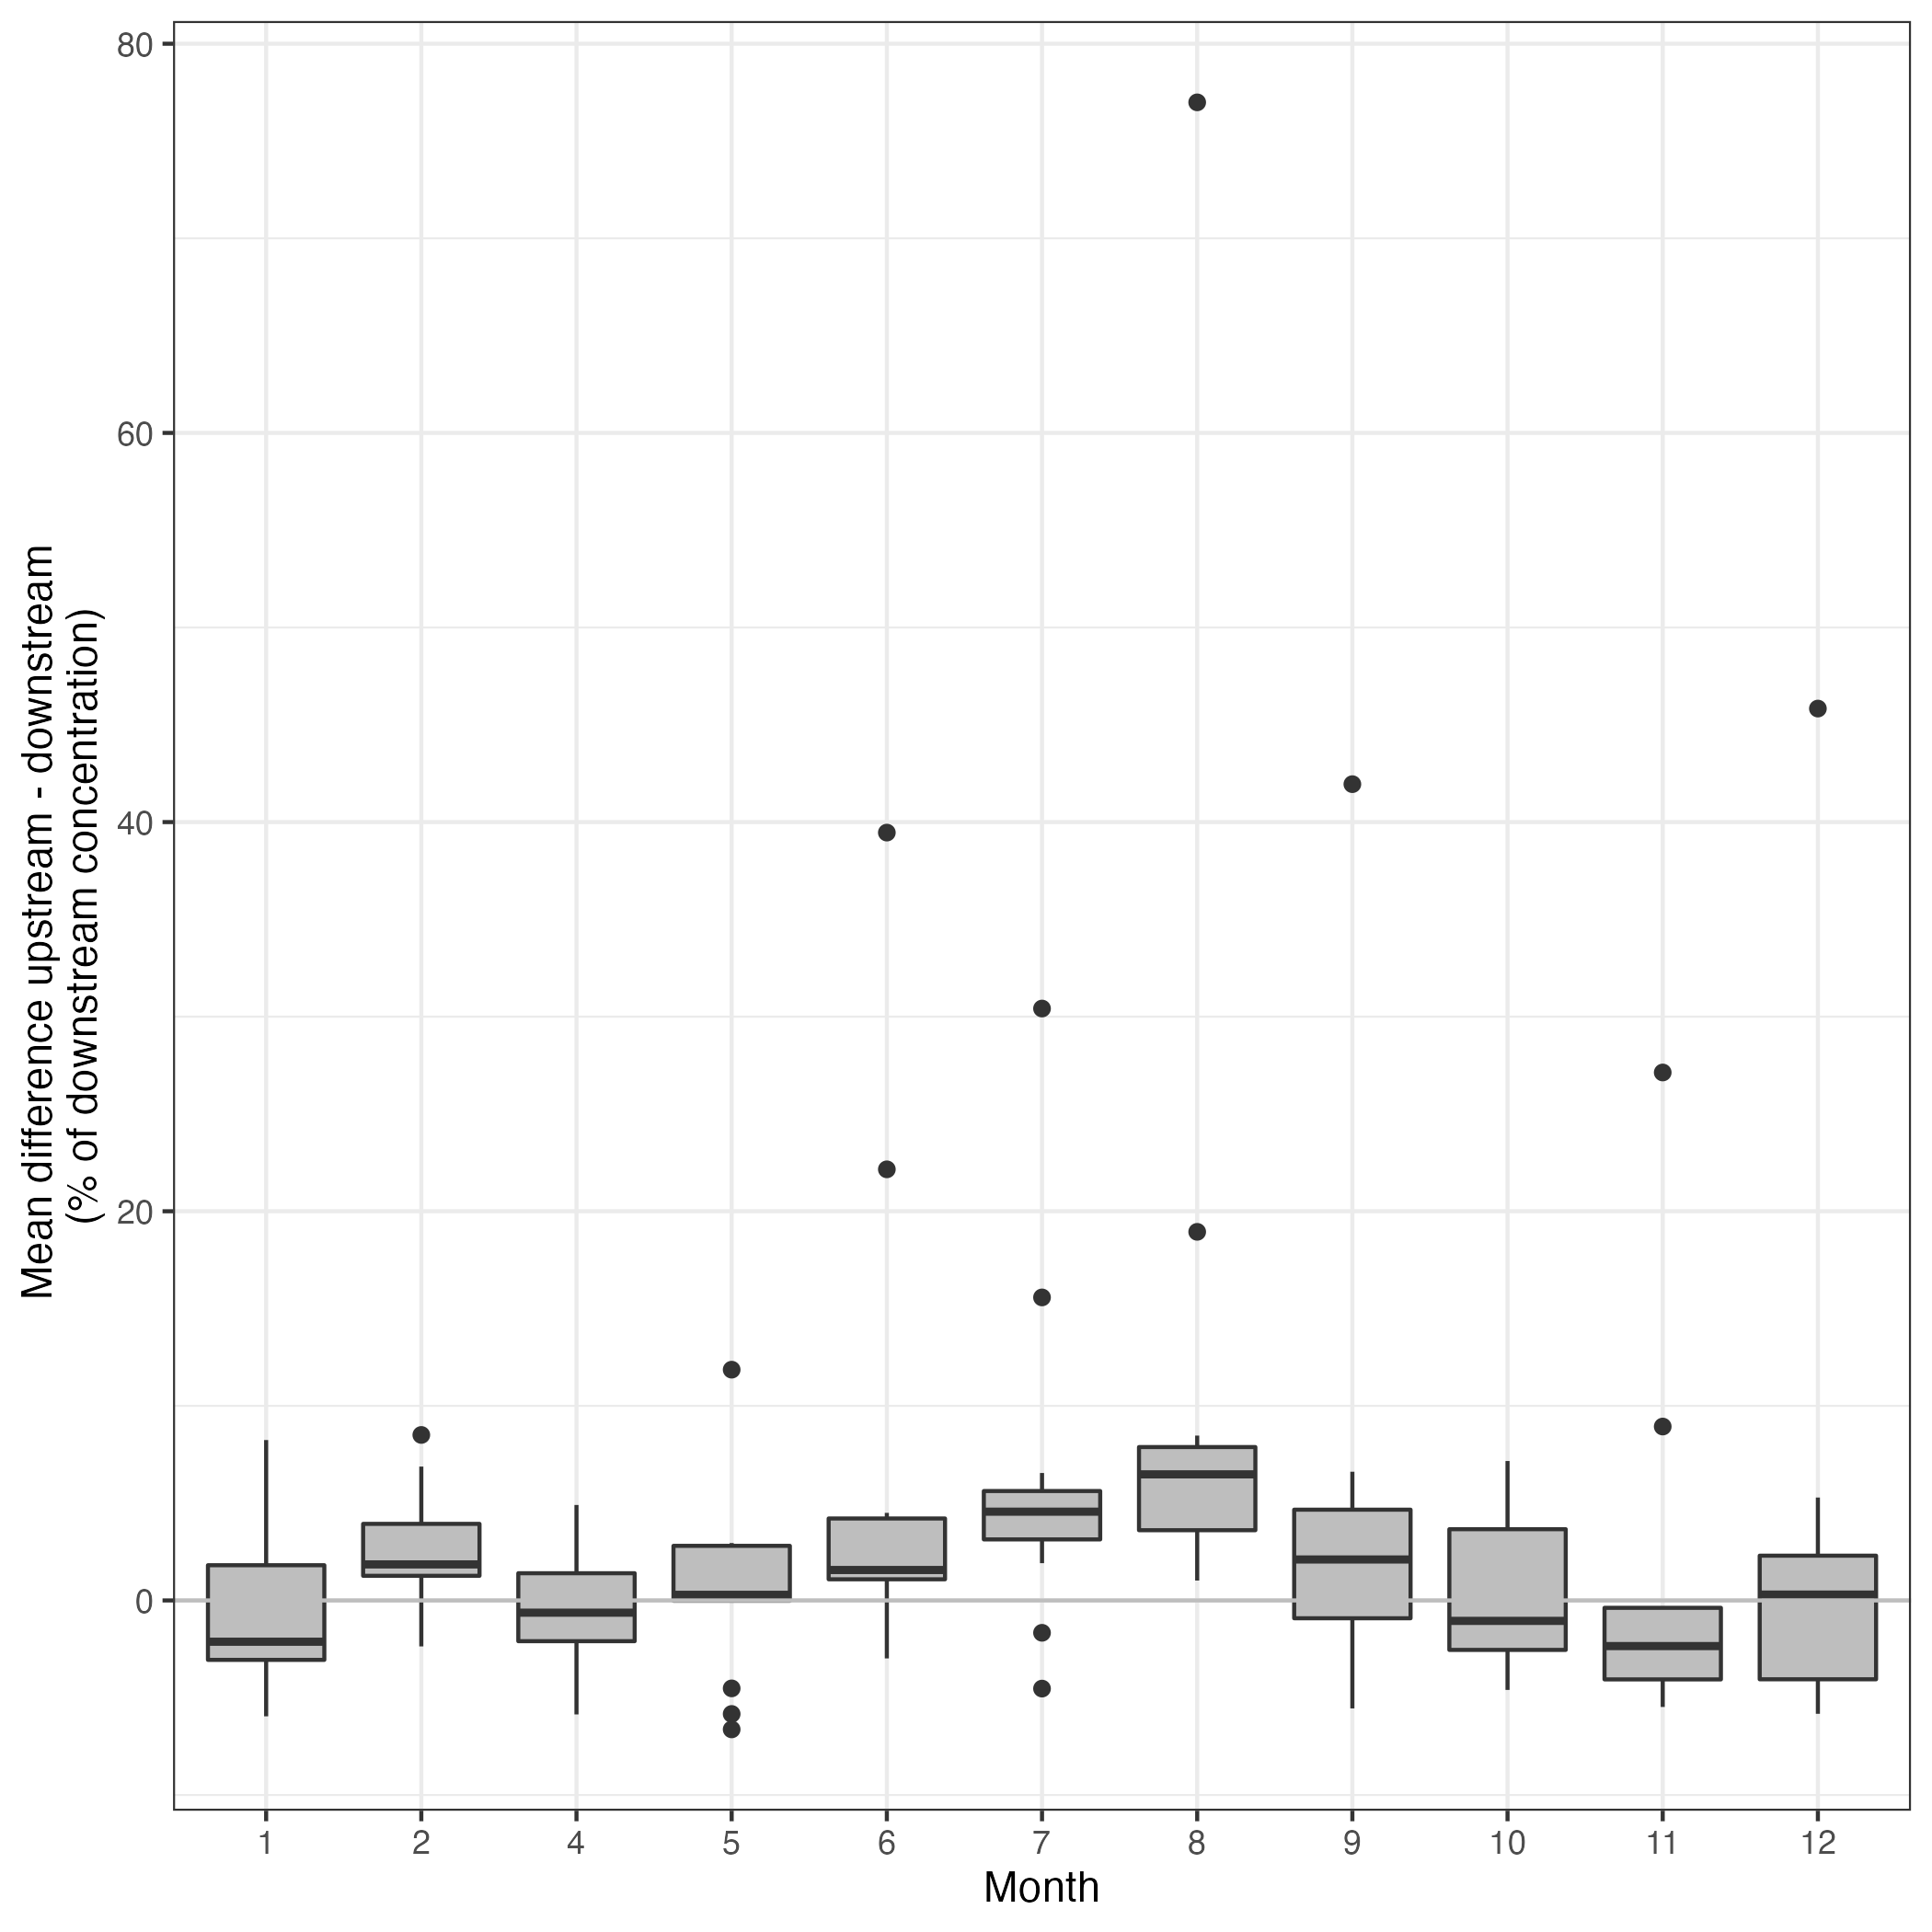
\includegraphics[width=0.6\textwidth,height=\textheight]{../Output/Figures/20221123_culvert_effect_flowcorrected.png}

The effects of the culvert-removal operation appear to have been
transient and fairly minor for the four salmonid species surveyed. After
the beginning of construction in September 2021 through the end of
sampling in February 2022, we see fluctuations in the percent changes of
salmonid DNA due to the culvert removal (Figure 7). \emph{O. clarkii} is
the least impacted species of the construction and \emph{O. nerka} and
\emph{O. mykiss} were the most impacted species, likely due to their
already low concentrations in the creek. For all species, a very slight
drop in concentration occurs in September and October (ca. 5-25\%
depending on the species), followed by an clear increase in November
(ca. 20-50\% depending on the species), and then a stabilization of the
concentration in December through February.

Of note, fish were exluded on August 30th, 2021 in preparation for the
stream to be diverted on September 9th, 2021 and the diversion was
removed October 7th, 2021. Water sampling occurred on September 10th,
2021, the day after the diversion, and on October 12, 2021, just 5 days
after reconnecting the stream (Supplemental Table X).

\begin{figure}
\centering
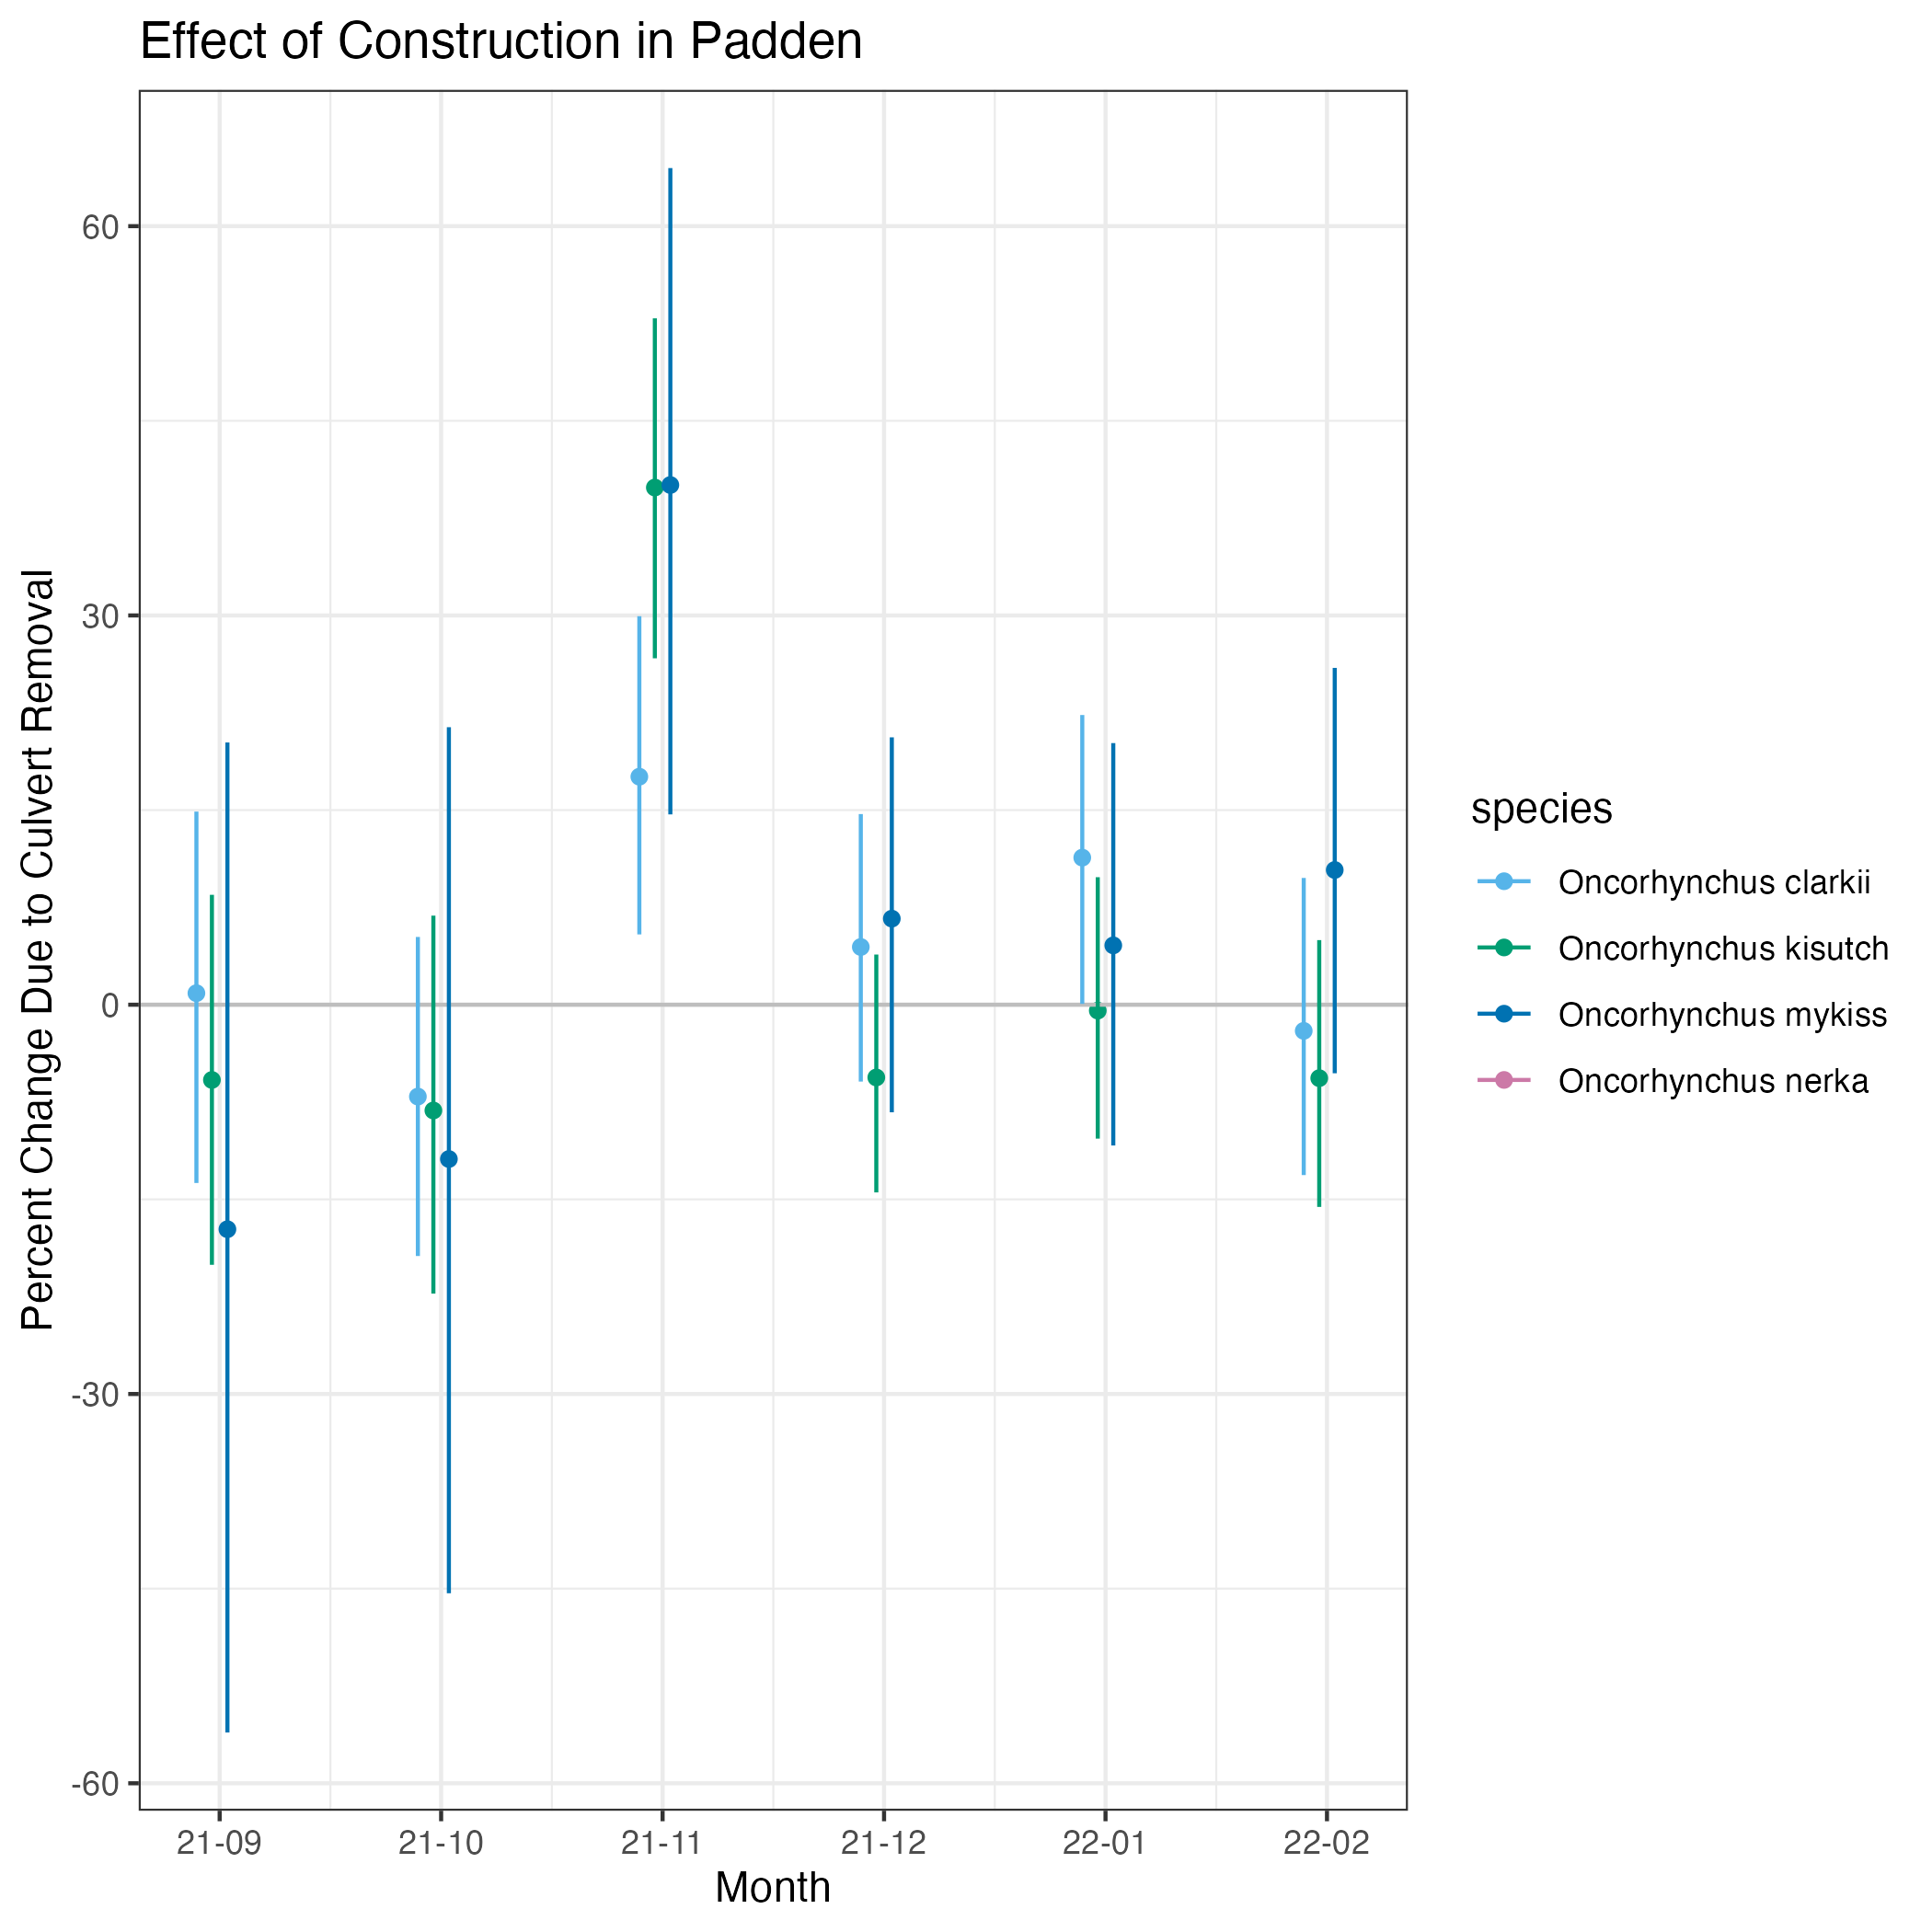
\includegraphics[width=0.6\textwidth,height=\textheight]{../Output/Figures/20221123_Construction_effect.png}
\caption{Effect of Construction on DNA Concentrations in Padden Creek.
Error bars show 95\% confidence intervals.}
\end{figure}

\hypertarget{discussion}{%
\subsection{Discussion}\label{discussion}}

\hypertarget{environmental-dna-can-provide-quantitative-measurements-of-environmental-impacts}{%
\subsubsection{Environmental DNA can provide quantitative measurements
of environmental
impacts}\label{environmental-dna-can-provide-quantitative-measurements-of-environmental-impacts}}

A clear seasonal pattern occurred for all the salmonids detected in the
study. The time series model uses shared information across creeks to
include the change in eDNA concentrations due to time, whether a sample
was collected below or above a barrier (i.e., culvert), and whether or
not there was construction occurring. Thus, we could isolate the changes
in eDNA concentrations as a result of the intervention (i.e.,
construction) while accounting for the variance due to time and station
(i.e., season and culvert).

Furthermore, we can use just one qPCR assay in combination with
metabarcoding data to get information about many more species without
running n qPCR assays for n species detected in metabarcoding data
(which is also particularly helpful for species that don't have a
previously published assay).

\hypertarget{not-all-culverts-are-barriers}{%
\subsubsection{Not all culverts are
barriers}\label{not-all-culverts-are-barriers}}

By measuring DNA concentrations of species above and below culverts on a
small spatial scale, we were able to determine how much of a barrier
each culvert was (or was not) to fish passage. We found that four of the
five creeks sampled did not seem to be major barriers to fish passage.
The only creek that was determined to be a barrier to fish passage was
Barnes Creek, as we only found salmonid DNA in three months of the
twelve months of sampling, and those three months had very low
conentration of salmonid DNA relative to the other creeks.

Of the creeks where salmonid DNA was consistently found, Chuckanut Creek
had the largest discrepancies between DNA concentrations found below and
above the barrier at each time point. The culvert in Chuckanut Creek is
suspected to be a barrier to fish passage and the State of Washington's
Department of Transportation (WSDOT) is planning to replace it in the
near future.

The culverts at Portage Creek and Squalicum Creek were more recently
installed as compared to Padden, Chuckanut, and Barnes Creeks. They also
were not designated by WSDOT as blocking fish passage. Squalicum Creek
had the lowest difference between upstream and downstream concentrations
across all the surveyed creeks. Portage Creek had a higher

\hypertarget{salmonids-can-survive-a-bulldozer-in-a-creek}{%
\subsubsection{Salmonids can survive a bulldozer in a
creek}\label{salmonids-can-survive-a-bulldozer-in-a-creek}}

The intervention (i.e., construction) in Padden Creek occurred over
about two months and included the ``de-watering'' of the creek, removal
of the existing culvert, installation of the new culvert, and then the
``re-watering'' of the creek from late August 2021 to October 2021. The
impact of the construction itself on salmonid species demonstrates an
initial decrease in DNA concentrations in September and October,
followed by a large increase in DNA concentration in November, and then
a stabilization and return to nearly baseline concentrations from
December to February. This pattern remarkably demonstrates an expected
response to a large intervention. During the actual construction, we
found less eDNA from salmonids, but after the completion of the
installing a new culvert, concentrations increased and then returned to
baseline.

The overall pattern of this effect was similar for the four species of
salmonids, but the species of which we found higher eDNA concentrations
seemed to have a dampened effect compared to the rarer species. This
also corresponds to species with different life histories and behaviors,
and it might be that our most commonly and abundant species, \emph{O.
clarkii}, was more robust to the intervention because it has both
migrating and non-migrating subspecies (see below).

\hypertarget{fish-migrations-and-expected-patterns}{%
\subsubsection{Fish migrations and expected
patterns}\label{fish-migrations-and-expected-patterns}}

Here, we consider four salmonid species to assess fish passage and the
impact of construction. These four species, and even individuals within
a species, have different behavior that would impact where fish might be
in the creeks and therefore eDNA concentrations. For example, within
cutthroat trout (\emph{O. clarkii}) there might be both non-migrating,
resident trout in the creeks and coastal run cutthroat that migrate into
Padden Creek from Bellingham Bay. Similarly, \emph{O. nerka} includes
both anadromous sockeye salmon and non-migrating kokanee salmon and
\emph{O. mykiss} includes both anadromous steelhead trout and
non-migrating rainbow trout.

For migratory salmonids, the run timings vary for each species. In the
Bellingham area, coastal cutthroat (\emph{O. clarkii}) are documented to
run throughout the entire year, whereas coho salmon (\emph{O. kisutch})
run timings are September to December, kokanee salmon (\emph{O. nerka})
run October to December, and steelhead trout (\emph{O. mykiss}) run
November to June.

Using eDNA, we cannot distinguish between the migrating and
non-migrating subspecies of \emph{O. clarkii}, \emph{O. nerka}, and
\emph{O. mykiss}. Therefore, our eDNA concentrations might reflect
contributions from both migrating and non-migrating individuals at any
given time point in the dataset. However, the metabarcoding data
demonstrates that in Padden Creek, there is a clear signal of \emph{O.
nerka} both upstream and downstream only in November 2021-2022 (and only
upstream in March 2021). This signal corresponds well with the
documented run timing of October to December.

For the other salmonids included in this study, \emph{O. kistuch} does
not have a non-migrating subspecies, but eDNA is found in months outside
of the expected run timing of September to December. This could
potentially be due to juveniles maturing and migrating in the creeks
after adults migrate during the run time up the creeks to spawn.
\emph{). mykiss} is also found nearly year-round in Padden Creek and
Chuckanut Creek, which could be contributions from migrating steelhead
(November to June), juveniles maturing and migrating, or from
residential rainbow trout. Though the \emph{O. mykiss} signal is found
year-round, the highest concentrations do seem to correspond with the
steelhead run timing.

\hypertarget{decoupling-of-edna-from-fish}{%
\subsubsection{Decoupling of eDNA from
fish}\label{decoupling-of-edna-from-fish}}

Though eDNA can move downstream with water flow, here, we were measuring
if culverts were barriers to fish moving upstream as we were focused on
the impact of culverts on migratory salmon. In our case, we were
comparing if downstream stations had higher DNA concentrations than
upstream stations as a result of fish being unable to get upstream.

Finally, it should be noted that Lake Padden, about 1.5 km upstream from
the sampling sites, was stocked with cutthroat trout in January 2021,
rainbow trout in April and May 2021, and kokanee salmon in May 2021.
Given that no sequencing reads in the metabarcoding data are found for
\emph{O. nerka} in May, the potential transport of eDNA downstream from
Lake Padden to the location of eDNA sampling is expected to be
negligible. Futhermore, Lake Padden is open for recreational fishing for
all of these species and managers have reported that most of the stocked
fish are caught soon after stocking {[}CITE WHO?{]}.

\hypertarget{accounting-for-flow-rates-with-edna-concentrations}{%
\subsubsection{Accounting for flow rates with eDNA
concentrations}\label{accounting-for-flow-rates-with-edna-concentrations}}

\hypertarget{conclusion}{%
\subsection{Conclusion}\label{conclusion}}

\end{document}
